\documentclass[10pt]{report}

\usepackage{stan-talks}

\begin{document}
\sf

% TITLE SLIDE
%
\vspace*{-12pt}
\noindent
\spc{\Large\bfseries \color{MidnightBlue}{Stan:}}
\\[3pt]
\spc{\large\bfseries \color{MidnightBlue}{Probabilistic Modeling
    \& Bayesian Inference}}
\\[12pt]
\noindent
\spc{\bfseries Development Team}
  \\[2pt]
  \spc{\footnotesize Andrew Gelman, \ \myemph{Bob Carpenter}, \ Daniel
    Lee, \ Ben Goodrich, }
  \\
  \spc{\footnotesize Michael Betancourt, \ Marcus Brubaker, \ Jiqiang
    Guo, \ Allen Riddell,}
  \\
  \spc{\footnotesize Marco Inacio, \ Jeffrey Arnold, \ \myemph{Mitzi Morris}, \
    Rob Trangucci,}
  \\
  \spc{\footnotesize Rob Goedman, \ Brian Lau, \, Jonah Sol Gabry, \
    Robert L.\ Grant, \ }
  \\
  \spc{\footnotesize Krzysztof Sakrejda, \ Aki Vehtari, \ Rayleigh
    Lei, \ Sebastian Weber, }
  \\
  \spc{\footnotesize Charles Margossian, \ Vincent Picaud, \ Imad
    Ali, \ \myemph{Sean Talts},}
  \\
  \spc{\footnotesize Ben Bales, \ Ari Hartikainen, \ Matthijs
    V\`ak\`ar, \ Andrew Johnson}
\\[-8pt] \noindent
  \spc{\small Stan 2.17 \ \footnotesize (November 2017)
    \hfill \url{http://mc-stan.org}} \hfill

\includegraphics[width=0.45in]{img/new-logo.png}


\sld{Stan's Namesake}
%
\begin{itemize}
\item Stanislaw Ulam (1909--1984)
\item Co-inventor of Monte Carlo method
\item[]
  \begin{center}
    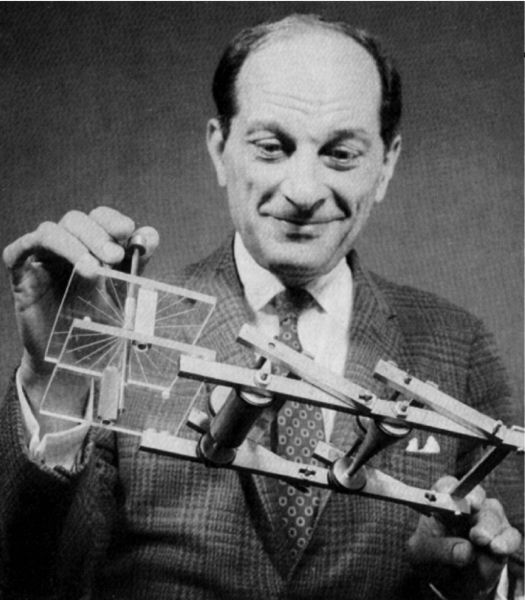
\includegraphics[width=0.25\textwidth]{img/ulam-fermiac.jpg}
  \end{center}
  {\small
  \item Ulam holding the Fermiac, Enrico Fermi's physical Monte Carlo simulator
    for random neutron diffusion}
\end{itemize}


\sld{Why Stan?}
%
\begin{itemize}
\item {\slshape\bfseries Application}: Fit rich Bayesian statistical models
\end{itemize}
%
\vspace*{2pt}
\begin{itemize}
\item {\slshape Problem}: Gibbs and Metropolis too slow (diffusive) 
\item {\slshape Solution}: Hamiltonian Monte Carlo (flow)
%
\vspace*{8pt}
\item {\slshape Problem}:  Interpreters slow and unscalable
\item {\slshape Solution}: Compiled to C++
%
\vspace*{8pt}
\item {\slshape Problem}:  Need gradients of log posterior for HMC
\item {\slshape Solution}: Reverse-mode algorithmic differentation
\end{itemize}


\sld{Why Stan? (cont.)}
%
\begin{itemize}
\item {\slshape Problem}:  Existing algo-diff slow, limited, unextensible
\item {\slshape Solution}: Our own algo-diff
%
\vspace*{8pt}
\item {\slshape Problem}:  Algo-diff requires functions templated on
  all args
\item {\slshape Solution}: Our own density library, Eigen linear
 algebra
%
\vspace*{8pt}
\item {\slshape Problem}:  Need unconstrained parameters for HMC
\item {\slshape Solution}: Variable transforms w. Jacobian determinants
%
\end{itemize}


\sld{Why Stan? (cont.)}
%
\begin{itemize}
\item {\slshape Problem}:  Need ease of use of BUGS
\item {\slshape Solution}: Compile a domain-specific language
%
\vspace*{8pt}
\item {\slshape Problem}:  Pure directed graphical language inflexible
\item {\slshape Solution}: Imperative probabilistic programming
  language
\vspace*{8pt}
\item {\slshape Problem}:  Need to tune parameters for HMC
\item {\slshape Solution}: Tune step size and estimate mass matrix
  during warmup;  on-the-fly number of steps (NUTS)
%
\end{itemize}


\sld{Why Stan? (cont.)}
%
\begin{itemize}
%
\vspace*{4pt}
\item {\slshape Problem}:  Efficient up-to-proportion density calcs
\item {\slshape Solution}: Density template metaprogramming 
%
\vspace*{4pt}
\item {\slshape Problem}:  Limited error checking, recovery
\item {\slshape Solution}: Static model typing, informative exceptions
%
\vspace*{4pt}
\item {\slshape Problem}:  Poor numerical stability
\item {\slshape Solutions}:
{
Taylor expansions, e.g., {\small \code{log1p()}}
\\[2pt]
compound functions, e.g., {\small \code{log\_sum\_exp()}, \
\code{BernoulliLogit()}}
\\[2pt]
limits at boundaries, e.g., {\small \code{multiply\_log()}}
}
%
\end{itemize}

\sld{Why Stan? (cont.)}
%
\begin{itemize}
\item {\slshape Problem}:  Nobody knows everything
\item {\slshape Solution}: Expand project team with specialists
\vspace*{8pt}
\item {\slshape Problem}:  Expanding code and project team
\item {\slshape Solution}: GitHub: branch, pull 
  request, code review
\item {\slshape Solution}: Jenkins: continuous integration
\item {\slshape Solution}: ongoing refactoring and code simplification
%
\end{itemize}

\sld{Why? (continued)}
\begin{itemize}
\item {\slshape Problem}:  Heterogeneous user base
\item {\slshape Solution}: More interfaces (R, Python, MATLAB, Julia)
\item {\slshape Solution}:  domain-specific examples, tutorials
\vspace*{8pt}
\item {\slshape Problem}:  Restrictive licensing limits use
\item {\slshape Solution}: Code and doc open source
(BSD, CC-BY)
\end{itemize}



\mypart{Prerequisite}{Bayesian Inference}


\sld{Bayesian Data Analysis}
%
\begin{itemize}
\item ``By {Bayesian data analysis}, we mean {practical methods}
  for making {inferences} from {data} using {probability models}
  for quantities we {observe} and about which we {wish to learn}.''
  % 
\item ``The essential characteristic of Bayesian methods is
  their \myemph{explict use of probability for quantifying uncertainty}
  in inferences based on statistical analysis.''
\end{itemize}
% 
\vfill\hfill{\footnotesize Gelman et al., {\slshape Bayesian Data Analysis},
  3rd edition, 2013}

\sld{Bayesian Methodology}
% 
\begin{itemize}
\item Set up \myemph{full probability model}
  \vspace*{-4pt}
  \begin{itemize}
  \item for all observable \& unobservable quantities
  \item consistent w. problem knowledge \& data collection
  \end{itemize}
  % 
\item \myemph{Condition} on observed data (where Stan comes in!)
  \vspace*{-4pt}
  \begin{itemize}
  \item to caclulate posterior probability of unobserved quantities
    (e.g., parameters, predictions, missing data)
  \end{itemize}
  % 
\item \myemph{Evaluate}
  \vspace*{-4pt}
  \begin{itemize}
  \item model fit and implications of posterior
  \end{itemize}
\vfill
\item \myemph{Repeat} as necessary
\end{itemize}
\vfill\hfill {\footnotesize {\slshape Ibid.}}


\sld{Where do Models Come from?}
%
\begin{itemize}
\item Sometimes model comes first, based on substantive
  considerations
\begin{subitemize}
\item toxicology, economics, ecology, physics, \ldots
\end{subitemize}
\item Sometimes model chosen based on data collection
\begin{subitemize}
\item  traditional statistics of surveys and experiments
\end{subitemize}
\item Other times the data comes first
\begin{subitemize}
\item observational studies, meta-analysis, \ldots
\end{subitemize}
\hfill
\item Usually its a mix
\end{itemize}


\sld{Model Checking}
%
\begin{itemize}
\item Do the inferences make sense?
\begin{subitemize}
\item are parameter values consistent with model's prior?
\item does simulating from parameter values produce reasoable fake
  data? 
\item are marginal predictions consistent with the data?
\end{subitemize}
\item Do predictions and event probabilities for new data make sense?
\vfill
\item {\slshape \myemph{Not}}: Is the model true?
\item {\slshape \myemph{Not}}: What is Pr[model is true]?
\item {\slshape \myemph{Not}}: Can we ``reject'' the model?
\end{itemize}


\sld{Model Improvement}
%
\begin{itemize}
\item Expanding the model
\begin{subitemize}
\item hierarchical and multilevel structure \ldots
\item more flexible distributions (overdispersion, covariance)
\item more structure (geospatial, time series)
\item more modeling of measurement methods and errors
\item \ldots
\end{subitemize}
\item Including more data
\begin{subitemize}
\item breadth (more predictors or kinds of observations)
\item depth (more observations)
\end{subitemize}
\end{itemize}


\sld{Properties of Bayesian Inference}
%
\begin{itemize}
\item Explores full range of parameters consistent with prior info and
  data$^*$
\begin{subitemize}
\item $^*$ if such agreement is possible
\item Stan automates this procedure with diagnostics
\end{subitemize}
\item Inferences can be plugged in directly for
\begin{subitemize}
\item parameter estimates minimizing expected error
\item predictions for future outcomes with uncertainty
\item event probability updates conditioned on data
\item risk assesment / decision analysis conditioned on uncertainty
\end{subitemize}
\end{itemize}


\sld{Notation for Basic Quantities}
% 
\begin{itemize}
\item \myemph{Basic Quantities}
\begin{subitemize}
\item $y$: \ observed data
\item $\theta$: \ parameters (and other unobserved quantities)
\item $x$: \ constants, predictors for conditional (aka ``discriminative'') models
\end{subitemize}
\item \myemph{Basic Predictive Quantities}
\begin{subitemize}
\item $\tilde{y}$: unknown, potentially observable quantities
\item $\tilde{x}$: \ constants, predictors for unknown quantities
\end{subitemize}
\end{itemize}


\sld{Naming Conventions}
%
\begin{itemize}
\item \myemph{Joint}: \ $p(y,\theta)$
\item \myemph{Sampling / Likelihood}: \ $p(y|\theta)$
\begin{subitemize}
\item Sampling is function of $y$ with $\theta$ fixed (prob function)
\item Likelihood is function of $\theta$ with $y$ fixed (\emph{not} prob function)
\end{subitemize}
\item \myemph{Prior}: \ $p(\theta)$
\item \myemph{Posterior}: \ $p(\theta|y)$
\item \myemph{Data Marginal (Evidence)}: \ $p(y)$
\item \myemph{Posterior Predictive}: \ $p(\tilde{y}|y)$
\end{itemize}


\sld{Bayes's Rule for Posterior}
% 
\vspace*{-4pt}
\begin{eqnarray*}
    p(\theta|y) 
    & = & \frac{p(y,\theta)}{p(y)} 
          \hspace*{64pt} \text{\small [def of conditional]}
    \\[6pt]
    & = & \frac{p(y|\theta) \, p(\theta)}{p(y)}
          \hspace*{44pt} \text{\small [chain rule]}
    \\[6pt]
    & = & \frac{p(y|\theta) \, p(\theta)}{\int_{\Theta} p(y,\theta') \ d\theta'}
          \hspace*{40pt} \text{\small [law of total prob]}
    \\[6pt]
    & = & \frac{p(y|\theta) \, p(\theta)}{\int_{\Theta} p(y|\theta') \,
      p(\theta') \ d\theta'}
          \hspace*{20pt} \text{\small [chain rule]}
\end{eqnarray*}
\vfill
\begin{itemize}
\item \emph{Inversion:} Final result depends only on 
  sampling distribution (likelihood) $p(y|\theta)$ and prior
  $p(\theta)$
\end{itemize}


\sld{Bayes's Rule up to Proportion}
%
\begin{itemize}
\item If data $y$ is fixed, then
\begin{eqnarray*}
p(\theta|y) 
& = & \frac{p(y|\theta) \, p(\theta)}{p(y)}
\\[6pt]
& \propto & p(y|\theta) \, p(\theta) 
\\[6pt]
& = & p(y,\theta)
\end{eqnarray*}
\item Posterior proportional to likelihood times prior
\item Equivalently, posterior proportional to joint
\vfill
\item The nasty integral for data marginal $p(y)$ goes away
\end{itemize}

\sld{Posterior Predictive Distribution}
\begin{itemize}
\item Predict new data $\tilde{y}$ based on observed data $y$
\item Marginalize parameters $\theta$ out of posterior and likelihood
\begin{eqnarray*}
p(\tilde{y} \mid y)
& = & \mathbb{E}[p(\tilde{y} | \theta) \mid Y = y]
\\[6pt]
& = &
\int p(\tilde{y} | \theta) \, p(\theta | y) \, d\theta.
\end{eqnarray*}
\item Weights predictions $p(\tilde{y}|\theta)$,
by posterior $p(\theta|y)$
\item Integral notation shorthand for sums and/or integrals
\end{itemize}


\sld{Event Probabilities}
%
\begin{itemize}
\item Events are fundamental probability bearing units which
\begin{subitemize}
\item are defined by sets of outcomes
\item which occur or not with some probability
\end{subitemize}
\item Events typically defined as conditions on random variables, e.g.,
\begin{subitemize}
\item $\theta_b > \theta_g$ for more boy births than girl births
\item $z_k = 1$ for team A beating team B in game $k$
\end{subitemize}
\end{itemize}


\sld{Event Probabilities, cont.}
%
\begin{itemize}
\item $\theta = (\theta_1, \ldots, \theta_N)$ is a sequence of
  random variables
\item $c$ is a condition on $\theta$,
  so that $c(\theta_1, \ldots, \theta_N) \in \{ 0, 1 \}$
\item Suppose $Y = y$ is some observed data
\item The probability that the event holds conditioned on the data is
  given by
%
\begin{eqnarray*}
\Prob{c(\theta_1, \ldots, \theta_N) | Y = y}
& = & \mathbb{E}[c(\theta_1,\ldots, \theta_N) \mid Y]
\\[6pt]
& = & \int c(\theta) \, p(\theta|y) \, \mathrm{d}\theta
\end{eqnarray*}
%
\item Not frequentist, because involves parameter probabilities
\end{itemize}


\mypart{Stan Example}{Repeated Binary Trials}


\sld{Stan Program}
%
\begin{stancode}
data {
  int<lower=0> N;                 // number of trials
  int<lower=0, upper=1> y[N];     // success on trial n
}
parameters {
  real<lower=0, upper=1> theta;   // chance of success
}
model {
  theta ~ uniform(0, 1);          // prior
  for (n in 1:N)
    y[n] ~ bernoulli(theta);      // likelihood
}
\end{stancode}

\sld{A Stan Program...}
%
\begin{itemize}
\item defines log (posterior) density up to constant, so...
\item equivalent to define log density directly:
\begin{stancode}
model {
  increment_log_prob(0);
  for (n in 1:N)
    increment_log_prob(log(theta^y[n])
                           * (1 - theta)^(1 - y[n])));
}
\end{stancode}
\item equivalent to (a) drop constant prior and (b) vectorize
  likelihood: 
\begin{stancode}
model {
  y ~ bernoulli(theta);
}
\end{stancode}
\end{itemize}


\sld{R: Simulate Data}
%
\begin{itemize}
\item Generate data
\begin{codein}
> theta <- 0.30;
> N <- 20;
> y <- rbinom(N, 1, 0.3);

> y
\end{codein}
\begin{codeout}
 [1] 1 1 1 1 0 0 0 0 1 1 0 0 1 0 0 0 0 0 0 1
\end{codeout}
\item Calculate MLE as sample mean from data
\begin{codein}
> sum(y) / N
\end{codein}
\begin{codeout}
[1] 0.4
\end{codeout}
\end{itemize}


\sld{RStan: Bayesian Posterior}
%
\begin{codein}
> library(rstan);

> fit <- stan("bern.stan",
              data = list(y = y, N = N));

> print(fit, probs=c(0.1, 0.9));
\end{codein}
\begin{codeout}
Inference for Stan model: bern.
4 chains, each with iter=2000; warmup=1000; thin=1; 
post-warmup draws per chain=1000,
total post-warmup draws=4000.

        mean se_mean   sd    10%    90% n_eff Rhat
theta   0.41    0.00 0.10   0.28   0.55  1580    1
\end{codeout}


\sld{RStan:  Full Bayes}

\begin{minipage}[t]{\textwidth}
\footnotesize
\begin{Verbatim}
> N <- 5;   y <- c(0,1,1,0,0);
> fit <- stan("bernoulli.stan", data = c("N", "y"));
> print(fit, digits=2)
\end{Verbatim}
%
\vspace*{1pt}
%
\begin{Verbatim}[fontshape=sl]
Inference for Stan model: bernoulli.
4 chains, each with iter=2000; warmup=1000; thin=1; 

        mean    se    sd   2.5%    50%  97.5%  n_eff  Rhat
theta  0.43  0.01  0.18   0.11   0.42   0.78   1229     1
lp__  -5.33  0.02  0.80  -7.46  -5.04  -4.78   1201     1
\end{Verbatim}
%
\vspace*{3pt}
%
\begin{Verbatim}
> hist( extract(fit)$theta )
\end{Verbatim}
\vspace*{-24pt}
\hfill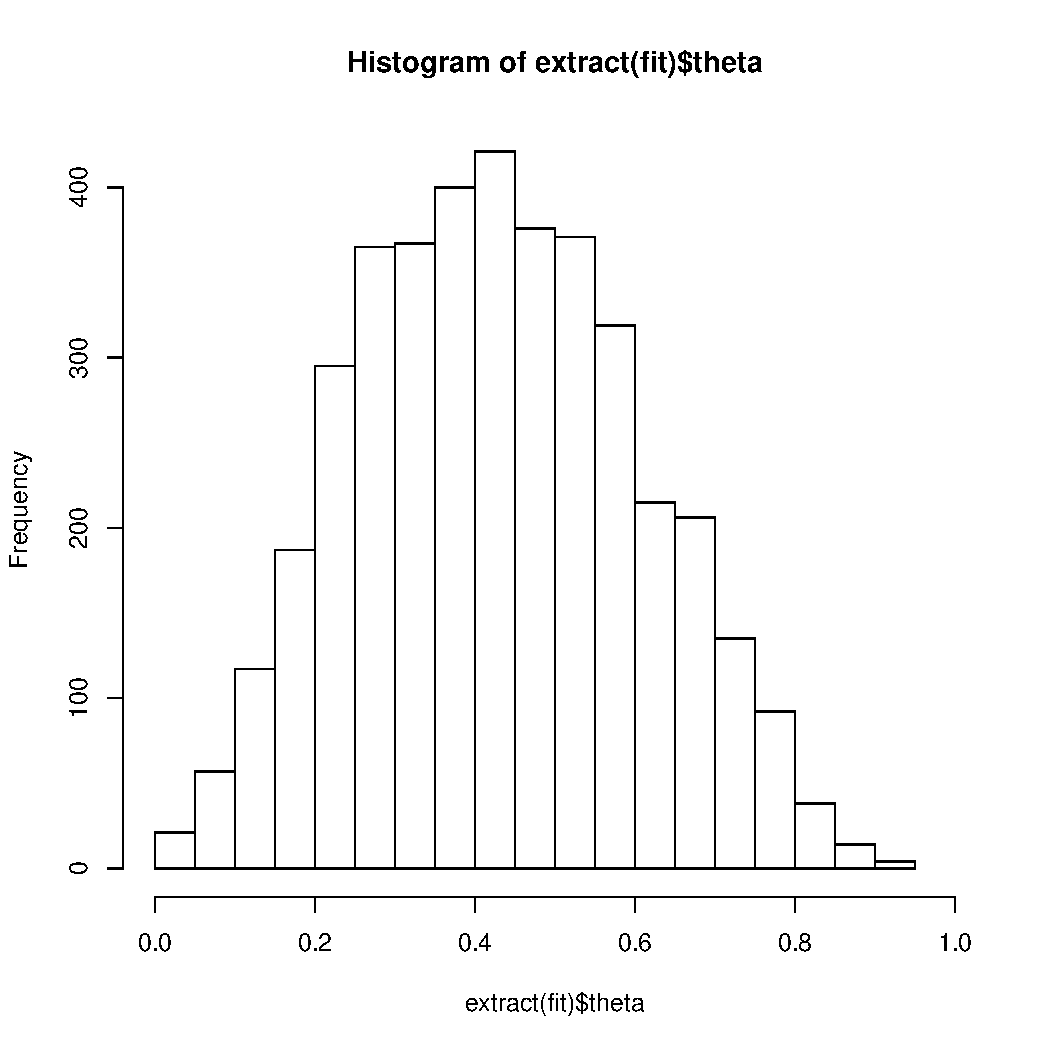
\includegraphics[height=0.9in]{img/bernoulli-posterior-histo.pdf}
\hspace*{24pt}
\end{minipage}


\sld{RStan: MAP, penalized MLE}

\begin{itemize}
\item Stan's optimization for estimation; two views:
\begin{subitemize}
\item max posterior mode, aka max a posteriori (MAP)
\item max penalized likelihood (MLE)
\end{subitemize}
\end{itemize}
\begin{center}
\begin{minipage}[t]{0.8\textwidth}\small
\begin{Verbatim}
> library(rstan);
> N <- 5;
> y <- c(0,1,1,0,0);
> model <- stan_model("bernoulli.stan");
> mle <- optimizing(model, data=c("N", "y"));
...
> print(mle, digits=2)
$par              $value  (log density)
theta             [1] -3.4
  0.4 
\end{Verbatim}
\begin{subitemize}
\item Posterior: $\distro{Beta}(1+2, 1+3)$;  mode $0.40$; mean $0.43$
\item Density: MLE w/o Jacobian;  MCMC with Jacobian
\end{subitemize}
\end{minipage}
\end{center}



\sld{Plug in Posterior Draws}
%
\begin{itemize}
\item Extracting the posterior draws
\begin{codein}
> theta_draws <- extract(fit)$theta;
\end{codein}
\item Calculating posterior mean (estimator)
\begin{codein}
> mean(theta_draws);
\end{codein}
\begin{codeout}
[1] 0.4128373
\end{codeout}
\item Calculating posterior intervals
\begin{codein}
> quantile(theta_draws, probs=c(0.10, 0.90));
\end{codein}
\begin{codeout}
      10%       90% 
0.2830349 0.5496858 
\end{codeout}
\end{itemize}


\sld{ggplot2: Plotting}
%
\begin{codein}
theta_draws_df <- data.frame(list(theta = theta_draws));
plot <-
  ggplot(theta_draws_df, aes(x = theta)) +
  geom_histogram(bins=20, color = "gray");
plot;
\end{codein}
\vspace*{-9pt}
\begin{center}
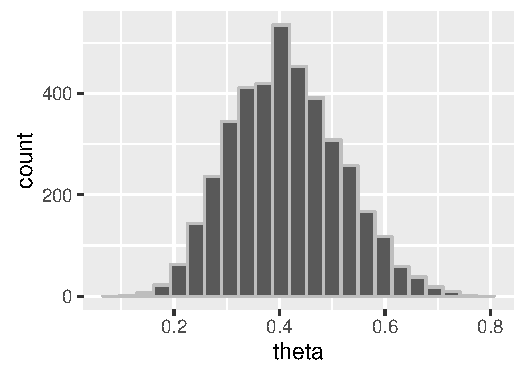
\includegraphics[height=1.45in]{img/bern-posterior-histogram.pdf}
\end{center}


\sld{Default Priors and Vectorization}
\begin{itemize}
\item All parameters are uniform by default
\item Probability functions can be vectorized (more efficient)
\item Thus
{\small
\begin{Verbatim}
      theta ~ uniform(0,1);
      for (n in 1:N) 
        y[n] ~ bernoulli(theta);
\end{Verbatim}
}
\mbox{ }
\\
{\normalsize reduces to}
\\
{\small
\begin{Verbatim}
      y ~ bernoulli(theta);
\end{Verbatim}
}
\end{itemize}


\mypart{Example}{Fisher "Exact" Test}


\sld{Bayesian ``Fisher Exact Test''}
%
\vspace*{-4pt}
\begin{itemize}
\item Suppose we observe the following data on handedness
\begin{center}
{\small
\begin{tabular}{c|c|c||c}
     & {\slshape sinister} & {\slshape dexter} & TOTAL
\\ \hline \hline
{\slshape male} & 9 ($y_1$) & 43 & 52 ($N_1$)
\\
{\slshape female} & 4 ($y_2$) & 44 & 48 ($N_2$)
\end{tabular}
}
\end{center}
\item Assume likelihoods $\distro{Binomial}(y_k|N_k,\theta_k)$, uniform
  priors
\item Are men more likely to be lefthanded?
{\small
\begin{eqnarray*}
\Prob{\theta_1 > \theta_2 \, | \, y, N}
& = & 
\int_{\Theta} \indicator{\theta_1 > \theta_2} \, p(\theta|y,N) \,
d\theta
\\[4pt]
& \approx & \frac{1}{M} \sum_{m=1}^M \indicator{\theta_1^{(m)} > \theta_2^{(m)}}.
\end{eqnarray*}
}
\end{itemize}


\sld{Stan Binomial Comparison}
%
\begin{stancode}
data {
  int y[2];
  int N[2];
}
parameters {
  vector<lower=0,upper=1> theta[2];
}
model {
  y ~ binomial(N, theta);
}
generated quantities {
  real boys_minus_girls = theta[1] - theta[2];
  int boys_gt_girls = theta[1] > theta[2];
}
\end{stancode}

\sld{Results}

\begin{codeout}
                   mean    2.5%  97.5%
theta[1]           0.22    0.12   0.35
theta[2]           0.11    0.04   0.21
boys_minus_girls   0.12   -0.03   0.26
boys_gt_girls      0.93    0.00   1.00
\end{codeout}
\begin{itemize}
\item 
$\mathrm{Pr}[\theta_1 > \theta_2 \,|\, y] \approx 0.93$
\item
$\mathrm{Pr}\left[
(\theta_1 - \theta_2) \in (-0.03, 0.26)
\,|\, y
\right] 
\, = \, 95\%$
\end{itemize}


\sld{Visualizing Posterior Difference}
%
\begin{itemize}
\item Plot of posterior difference, $p(\theta_1 - \theta_2 \, | \, y,
  N)$ (men - women)
\begin{center}
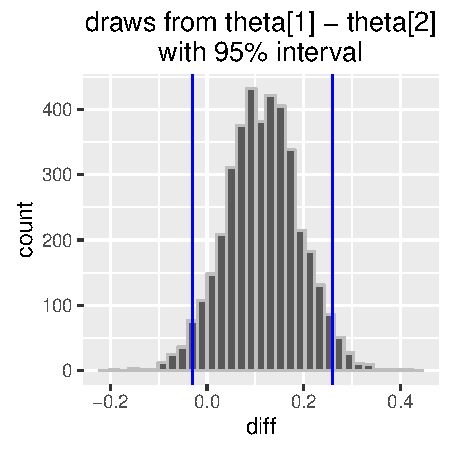
\includegraphics[height=1.65in]{img/lefty-posterior.pdf}
\end{center}
\item Vertical bars: central 95\% posterior interval $(-0.03,0.26)$
\end{itemize}


\mypart{Example}{More Stan Models}


\sld{Posterior Predictive Distribution}
%
\begin{itemize}
\item Predict new data ($\tilde{y}$) given observed data ($y$)
\item Includes two kinds of uncertainty
\begin{subitemize}
\item parameter estimation uncertainty: $p(\theta | y)$
\item sampling uncertainty:  $p(\tilde{y} | \theta)$
\end{subitemize}
\vspace*{-8pt}\begin{eqnarray*}
p(\tilde{y} |  y)
& = & \int p(\tilde{y} | \theta)
           \ p(\theta | y)
           \ \mathrm{d}\theta
\\[4pt]
& \approx & \frac{1}{M} \sum_{m=1}^M p(\tilde{y} | \theta^{(m)})
\end{eqnarray*}
\item Can generate predictions as sample of draws $\tilde{y}^{(m)}$
  based on $\theta^{(m)}$
\end{itemize}


\sld{Posterior Predictive Inference}
%
\begin{itemize}
\item Parameters $\theta$, observed data $y$, and data to predict $\tilde{y}$
\[
p(\tilde{y}|y) = \int_{\Theta} p(\tilde{y}|\theta) \ p(\theta|y) \ d\theta
\]
\item 
{\small
\begin{Verbatim}
data {
  int<lower=0> N_tilde;
  matrix[N_tilde,K] x_tilde;
  ...
parameters {
  vector[N_tilde] y_tilde;
  ...
model {
  y_tilde ~ normal(x_tilde * beta, sigma);
\end{Verbatim}
}
\end{itemize}


\sld{Predict w.\ Generated Quantities}
%
\begin{itemize}
\item Replace sampling with pseudo-random number generation
{\footnotesize
\begin{Verbatim}
   generated quantities {
     vector[N_tilde] y_tilde;

     for (n in 1:N_tilde) 
       y_tilde[n] <- normal_rng(x_tilde[n] * beta, sigma);
   }
\end{Verbatim}
}
\item Must include noise for predictive uncertainty
\item PRNGs only allowed in generated quantities block
\begin{subitemize}
\item more computationally efficient per iteration
\item more statistically efficient with i.i.d.\ samples \\
(i.e., MC, not MCMC)
\end{subitemize}
\end{itemize}


\sld{Linear Regression with Prediction}
%
\begin{stancode}
data {
  int<lower=0> N;               int<lower=0> K;
  matrix[N, K] x;               vector[N] y;
  matrix[N_tilde, K] x_tilde;
}
parameters {
  vector[K] beta;               real<lower=0> sigma;
}
model {
  y ~ normal(x * beta, sigma);
}
generated quantities {
  vector[N_tilde] y_tilde
    = normal_rng(x_tilde * beta, sigma);
}
\end{stancode}


\sld{Transforming Precision}
%
\begin{stancode}
    parameters {
      real<lower=0> tau;      // precision
      ...
    }
    transformed parameters {
      real<lower=0> sigma;    // scale
      sigma <- 1 / sqrt(tau);
    }
\end{stancode}


\sld{Logistic Regression}
%
\begin{stancode}
     data {
       int<lower=1> K;
       int<lower=0> N;
       matrix[N,K] x;
       int<lower=0,upper=1> y[N];
     }
     parameters {
       vector[K] beta;
     }
     model {
        beta ~ cauchy(0, 2.5);          // prior
        y ~ bernoulli_logit(x * beta);  // likelihood
     }
\end{stancode}


\sld{Generalized Linear Models}
%
\begin{itemize}
\item Direct parameterizations more efficient and stable
\item \myemph{Logistic regression} (boolean/binary data)
\begin{subitemize}
\item \Verb|y ~ bernoulli(inv_logit(eta));|
\item \Verb|y ~ bernoulli_logit(eta);|
\item Probit via \code{Phi} (normal cdf)
\item Robit (robust) via Student-$t$ cdf
\end{subitemize}
\item \myemph{Poisson regression} (count data)
\begin{subitemize}
\item \Verb|y ~ poisson(exp(eta));|
\item \Verb|y ~ poisson_log(eta);|
\item Overdispersion with negative binomial
\end{subitemize}
\end{itemize}


\sld{GLMS, continued}
%
\begin{itemize}
\item \myemph{Multi-logit regression} (categorical data)
\begin{subitemize}
\item \Verb|y ~ categorical(softmax(eta));|
\item \Verb|y ~ categorical_logit(eta);|
\end{subitemize}
\item \myemph{Ordinal logistic regression} (ordered data)
\begin{subitemize}
\item Add cutpoints \code{c}
\item \Verb|y ~ ordered_logistic(eta, c);|
\end{subitemize}
\item \myemph{Robust linear regression} (overdispersed noise)
\begin{subitemize}
\item \Verb|y ~ student_t(nu, eta, sigma);|
\end{subitemize}
\end{itemize}


\sld{Time Series Autoregressive: AR(1)}
%
\begin{stancode}
  data {
    int<lower=0> N;   vector[N] y;
  }
  parameters {
    real alpha;  real beta;  real sigma;
  } 
  model {
    y[2:n] ~ normal(alpha + beta * y[1:(n-1)], sigma);
  }
\end{stancode}


\sld{LKJ Density and Cholesky Factors}
%
\begin{itemize}
\item Density on \emph{correlation} \ matrices $\Omega$
%
\item $\distro{LKJCorr}(\Omega \, | \, \nu) 
       \propto \mbox{det}(\Omega)^{(\nu - 1)}$
\begin{subitemize}
\item $\nu = 1$ uniform
\item $\nu > 1$ concentrates around unit matrix
\end{subitemize}
%
\item Work with Cholesky factor $L_{\Omega}$ s.t. $\Omega = L_{\Omega} \, L_{\Omega}^{\top}$
\begin{subitemize}
\item Density: $\distro{LKJCorrCholesky}(L_{\Omega} \, | \, \nu)
\propto |J| \, \mbox{det}(L_{\Omega} \, L_{\Omega}^{\top})^{(\nu - 1)}$ 
\item Jacobian adjustment for Cholesky factorization
\end{subitemize}
%
\end{itemize}
\vfill
\hfill {\footnotesize Lewandowski, Kurowicka, and Joe (2009)}


\sld{Covariance Random-Effects Priors}
%
\vspace*{-4pt}
{\footnotesize
\begin{Verbatim}
    parameters {
      vector[2] beta[G];  
      cholesky_factor_corr[2] L_Omega;
      vector<lower=0>[2] sigma;

    model {
      sigma ~ cauchy(0, 2.5);
      L_Omega ~ lkj_cholesky(4);
      beta ~ multi_normal_cholesky(rep_vector(0, 2),
                             diag_pre_multiply(sigma, L_Omega));
      for (n in 1:N)
        y[n] ~ bernoulli_logit(... + x[n] * beta[gg[n]]);
\end{Verbatim}
}
\vspace*{6pt}
\begin{subitemize}
\item $G$ groups with varying slope and intercept; \code{gg} indicates group
\end{subitemize}


\sld{Multivariate Random-Effects Priors}
%
\begin{stancode}
parameters {
  vector[2] beta[G];  
  cholesky_factor_corr[2] L_Omega;
  vector<lower=0>[2] sigma;
  ...
model {
  sigma ~ cauchy(0, 2.5);
  L_Omega ~ lkj_cholesky(4);
  beta ~ multi_normal_cholesky(rep_vector(0, 2),
                         diag_pre_multiply(sigma, L_Omega));
  for (n in 1:N)
    y[n] ~ bernoulli_logit(... + x[n] * beta[gg[n]]);
\end{stancode}


\sld{\large Example: Gaussian Process Estimation}
%
\vspace*{-5pt}
\begin{stancode}
data {
  int<lower=1> N;  vector[N] x; vector[N] y;
} parameters {
  real<lower=0> eta_sq, inv_rho_sq, sigma_sq;
} transformed parameters {
  real<lower=0> rho_sq; rho_sq <- inv(inv_rho_sq);
} model {
  matrix[N,N] Sigma;
  for (i in 1:(N-1)) { 
    for (j in (i+1):N) {
      Sigma[i,j] <- eta_sq * exp(-rho_sq * square(x[i] - x[j]));
      Sigma[j,i] <- Sigma[i,j];
  }}
  for (k in 1:N) Sigma[k,k] <- eta_sq + sigma_sq;
  eta_sq, inv_rho_sq, sigma_sq ~ cauchy(0,5);
  y ~ multi_normal(rep_vector(0,N), Sigma);
}
\end{stancode}


\sld{\large Gaussian Process Predictions}
%
\begin{itemize}
\item Add predictors \code{x\_tilde[M]} for points to predict
\item Declare predicted values \code{y\_tilde[M]} as unconstrained parameters
\item Define \code{Sigma[M+N,M+N]} in terms of full \code{append\_row(x, x\_tilde)}
\item Model remains the same
{\small
\begin{Verbatim}
 append_row(y,y_tilde)
   ~ multi_normal(rep(0,N+M),Sigma);
\end{Verbatim}
}
\end{itemize}


\sld{Non-Centered Parameterization}
%
\begin{stancode}
parameters {
  vector[K] beta_std;  // non-centered
  real mu;
  real<lower=0> sigma;
}
transformed parameters {
  vector[K] beta = mu + sigma * beta_raw;
}
model {
  mu ~ cauchy(0, 2.5);
  sigma ~ cauchy(0, 2.5);
  beta_std ~ normal(0, 1);
}
\end{stancode}


\sld{Mixture of Two Normals}
%
{\footnotesize
\begin{Verbatim}
        for (n in 1:N) {
          real lp1;  real lp2;

          lp1 <- bernoulli_log(0, lambda)               
                   + normal_log(y[n], mu[1], sigma[1]); 

          lp2 <- bernoulli_log(1, lambda)
                   + normal_log(y[n], mu[2], sigma[2]);

          increment_log_prob(log_sum_exp(lp1,lp2));  
\end{Verbatim}
}
\vspace*{2pt}
\begin{subitemize}
\item local variables reassigned; direct increment of log posterior
\item $\mbox{\rm log\_sum\_exp}(\alpha,\beta) = \log (\exp(\alpha) + \exp(\beta))$
\item \myemph{Much more efficient} than sampling (Rao-Blackwell Theorem)
\vspace*{10pt}
\end{subitemize}


\sld{Other Mixture Applications}
%
\begin{itemize}
\item Other multimodal data
\item Zero-inflated Poisson or hurdle models
\item Model comparison or mixture
\item Discrete change-point model
\item Hidden Markov model, Kalman filter
\item Almost anything with latent discrete parameters
\hfill
\item Other than variable choice, e.g., regression predictors
\begin{subitemize}
\item marginalization is exponential in number of vars
\end{subitemize}
\end{itemize}


\sld{Dynamic Systems with Diff Eqs}
%
\begin{itemize}
\item Simple harmonic oscillator
{\small
\begin{equation*}
\frac{d}{dt} y_1 = -y_2 
\hspace*{0.5in}
\frac{d}{dt} y_2 = -y_1 - \theta y_2
\end{equation*}
}
\item Code as a function in Stan
\end{itemize}
{\footnotesize
\begin{Verbatim}
        functions {
          real[] sho(real t, real[] y, real[] theta,
                     real[] x_r, int[] x_i) {
            real dydt[2];
            dydt[1] <- y[2];
            dydt[2] <- -y[1] - theta[1] * y[2];
            return dydt;
          }
        }
\end{Verbatim}
}


\sld{Fit Noisy State Measurements}

{\footnotesize
\begin{Verbatim}
    data {
      int<lower=1> T;      real y[T,2];
      real t0;             real ts[T];
    }
    parameters {
      real y0[2];                // unknown initial state
      real theta[1];             // rates for equation
      vector<lower=0>[2] sigma;  // measurement error
    }
    model {
      real y_hat[T,2];
      ...priors...
      y_hat <- integrate_ode(sho, y0, t0, ts, theta, x_r, x_i);
      for (t in 1:T)
        y[t] ~ normal(y_hat[t], sigma);
    }
\end{Verbatim}
}




\mypart{Overview}{What is Stan?}


\sld{What is Stan?}
%
\begin{itemize}
\item Stan is an \myemph{imperative} probabilistic programming language
\vspace*{-12pt}
  \begin{subitemize}
  \item  cf., BUGS: declarative; \ Church: functional; \ Figaro: object-oriented
  \end{subitemize}
\item Stan \myemph{program}
  \begin{subitemize}
  \item declares data and (constrained) parameter variables
  \item defines log posterior (or penalized likelihood)
  \end{subitemize}
\item Stan \myemph{inference}
  \begin{subitemize}
  \item MCMC for full Bayesian inference
  \item VB for approximate Bayesian inference
  \item MLE for penalized maximum likelihood estimation
  \end{subitemize}
\end{itemize}


\sld{Platforms and Interfaces}
%
\vspace*{-2pt}
\begin{itemize}
\item \myemph{Platforms}:  Linux, Mac OS X, Windows
\item \myemph{C++ API}: {\small portable, standards compliant (C++03;
    C++11 soon)}
\item \myemph{Interfaces}
\begin{subitemize}\footnotesize
  \item \myemph{CmdStan}: Command-line or shell interface (direct executable)
  \item \myemph{RStan}: R interface (Rcpp in memory)
  \item \myemph{PyStan}: Python interface (Cython in memory)
  \item \myemph{MatlabStan}: MATLAB interface (external process)
  \item \myemph{Stan.jl}: Julia interface (external process)
  \item \myemph{StataStan}: Stata interface (external process)
  \item \myemph{MathematicaStan}: Stata interface (external process)
\end{subitemize}
\end{itemize}


\sld{Higher-Level Interfaces}
%
\begin{itemize}
\item \myemph{R Interfaces}
\begin{subitemize}
 \item \myemph{RStanArm}: regression modeling with R expressions
 \item \myemph{ShinyStan}: web-based posterior visualization, exploration
 \item \myemph{Loo}:  approximate leave-one-out cross-validation
\end{subitemize}
\item \myemph{Jupyter Containers}
\begin{subitemize}
\item \myemph{Docker} versions for R, Python, Julia
\item \myemph{SageMath}: free online server (R)
\end{subitemize}
\item From others
\begin{subitemize}
\item \myemph{Prohet} (Facebook): time-series analysis (R and Python)
\item \myemph{brms} (B\"urkner): regression modeling with R expressions
\item \myemph{rethinking} (McElreath): simplified Stan embedded in R
\end{subitemize}
\end{itemize}
\vfill


\sld{Who's Using Stan?}
%
\begin{itemize}
\item 2500+ \myemph{users group} registrations;  20,000+ \myemph{downloads}
  \small{(per version just in Rstudio)}; 1000+ Google scholar citations
\item \myemph{Biological sciences}: {\footnotesize
clinical drug trials, entomology, pharmacology, toxicology, botany,
neurology, genomics, agriculture, botany, fisheries, genomics, cellular
biology, epidemiology, population ecology, neurology
}
\item \myemph{Physical sciences}: {\footnotesize
astrophysics, particle physics, molecular biology, oceanography, climatology, biogeochemistry, materials science
}
\item \myemph{Social sciences}: {\footnotesize
 econometrics (macro and micro), population dynamics, cognitive
 science, psycholinguistics, social networks, political science,
 survey sampling
}
\item \myemph{Other}: {\footnotesize materials engineering, finance,
    actuarial science, sports, public health, recommender systems,
    educational testing, fleet maintenance, sports}
\end{itemize}


\sld{Documentation}
%
\begin{itemize}
\item {\slshape Stan User's Guide and Reference Manual}
\begin{subitemize}
\item 600+ pages
\item example models, modeling and programming advice
\item introduction to Bayesian and frequentist statistics
\item complete language specification and execution guide
\item descriptions of algorithms (NUTS, R-hat, n\_eff)
\item guide to built-in distributions and functions
\end{subitemize}
\item Installation and getting started manuals by interface
\begin{subitemize}
\item RStan, PyStan, CmdStan, MatlabStan, Stan.jl, StataStan, MathematicaStan
\end{subitemize}
\item Many written and video tutorials by users and developers
\end{itemize}


\sld{Model Sets Translated to Stan}
%
\begin{itemize}
\item BUGS examples (most of all 3 volumes)
\item Gelman and Hill (2009) {\slshape Data Analysis Using Regression and
    Multilevel/Hierarchical Models}.
\item Wagenmakers and Lee (2014) {\slshape Bayesian Cognitive
    Modeling}.
\item K\'ery and Schaub (2014) {\slshape Bayesian Population Analysis
    Using WinBUGS}.
\item Kruschke (2014) {\slshape Doing Bayesian Data Analysis}.
\end{itemize}


\sld{Books about Stan}
%
\begin{subitemize}
\footnotesize
\item Gelman and Hill (2018) {\slshape Regression and Other Stories}. Cambridge.
\item Hilbe, de Souza, and Ishida (2017) {\slshape Bayesian Models for Astrophysical Data Using R, JAGS, Python, and Stan}. Cambridge.
\item Matsuura (2016) {\slshape Bayesian Statistical Modeling Using Stan and R}. Kyoritsu. (Japanese)
\item Faraway (2016) {\slshape Extending the Linear Model with R: Generalized Linear, Mixed Effects and Nonparametric Regression Models}, 2nd Edition. CRC.
\item McElreath (2016) {\slshape Statistical Rethinking: A Bayesian course
    with R and Stan}. CRC.
\item Korner-Nievergelt et al. (2015) {\slshape Bayesian Data Analysis in
    Ecology Using Linear Models with R, BUGS, and Stan}. Academic Press.
\item Kruschke (2014) {\slshape Doing Bayesian Data Analysis, Second
    Edition: A Tutorial with R, JAGS, and Stan}. Academic Press.
\item Gelman et al. (2013) {\slshape Bayesian Data Analysis}, 3rd Edition. CRC.
\end{subitemize}


\sld{Scaling and Evaluation}
%
\begin{center}
\vspace*{-6pt}
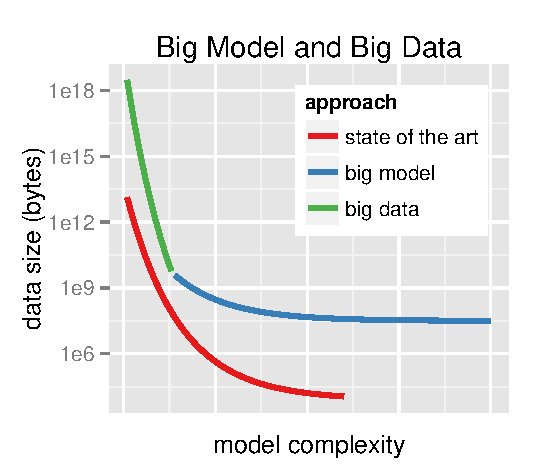
\includegraphics[width=0.4\textwidth]{img/big-model-big-data.pdf}
\vspace*{-6pt}
\end{center}
\begin{itemize}
\item Types of Scaling: data, parameters, \myemph{models}
\item Time to converge and per effective sample size: \\[2pt]
\mbox{ } \ \ \ {0.5--{\large$\infty$} times faster than BUGS \& JAGS}
\item Memory usage: \ {1--10\% of BUGS \& JAGS}
\end{itemize}


\sld{NUTS vs.\ Gibbs and Metropolis}
%
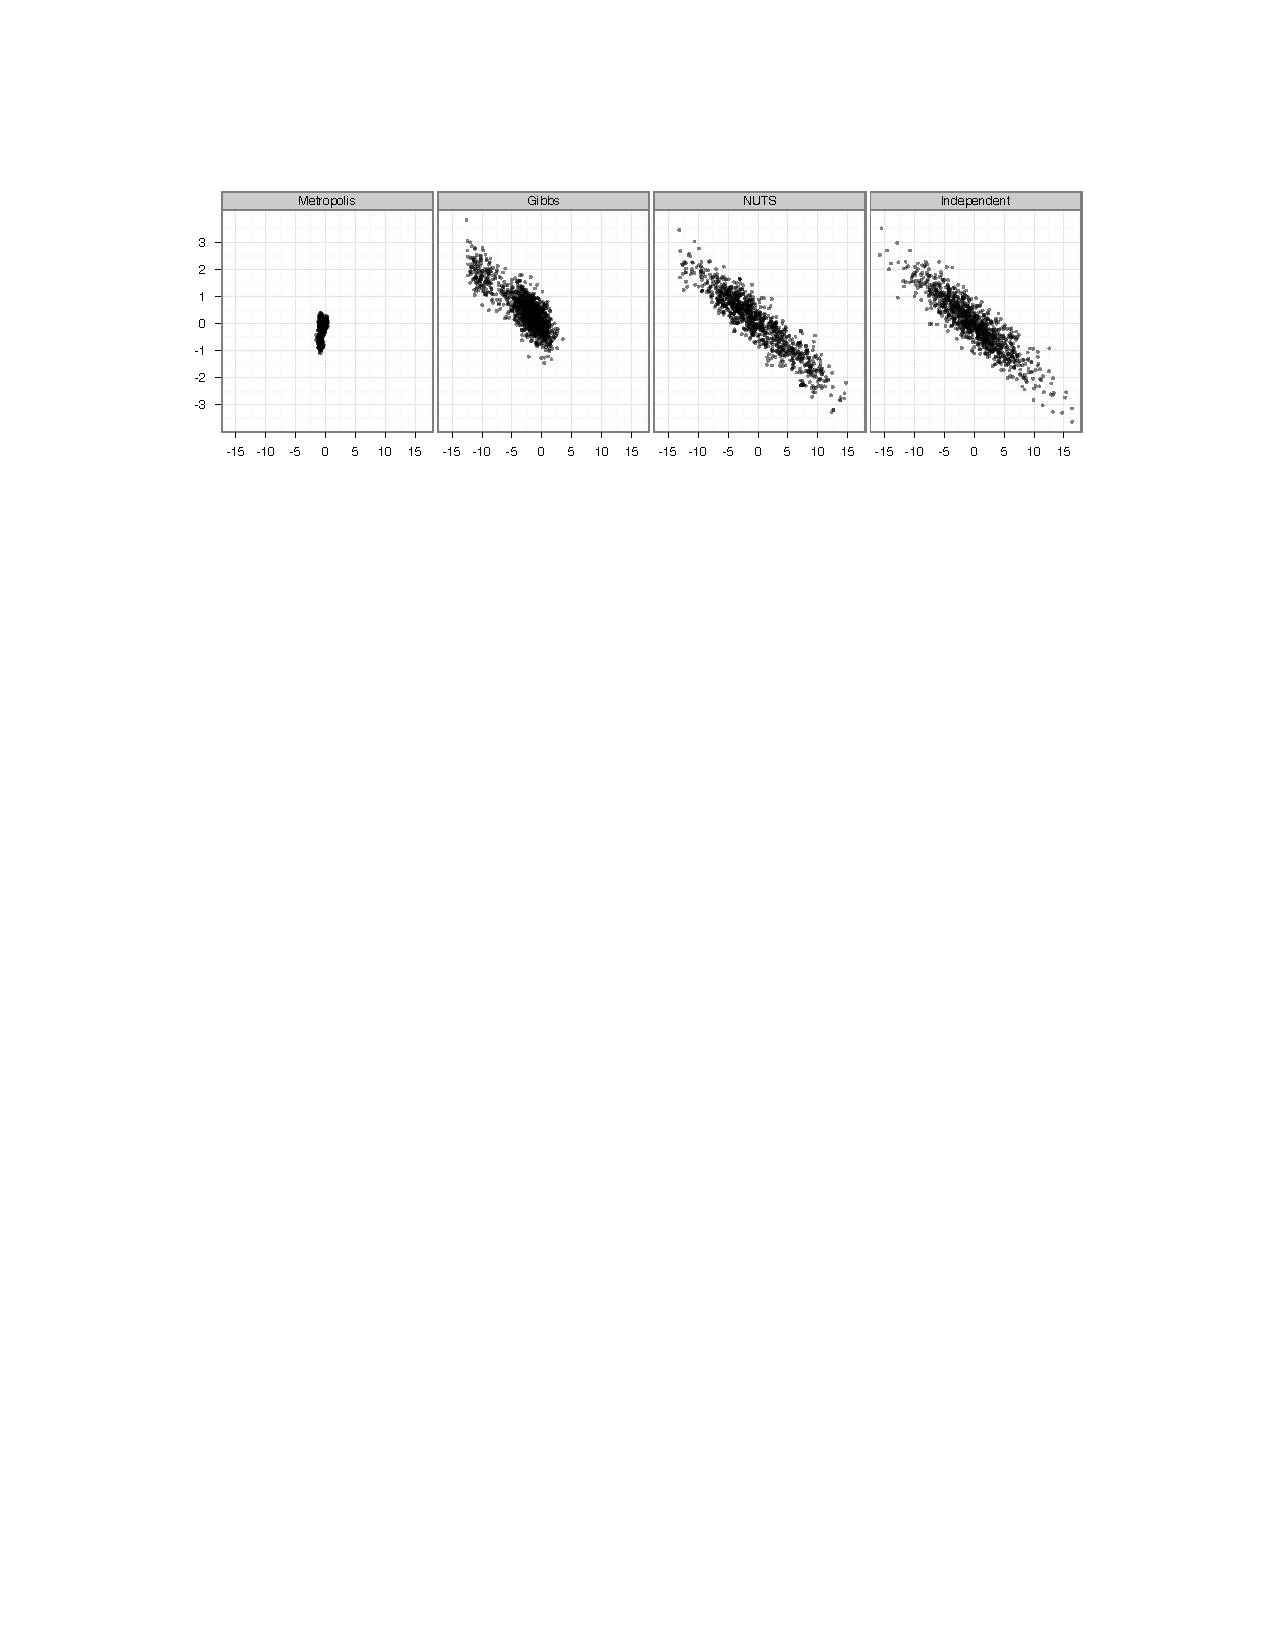
\includegraphics[width=0.9\textwidth]{img/nuts-vs.pdf}
\begin{subitemize}
\item Two dimensions of highly correlated 250-dim normal
\item \myemph{1,000,000 draws} from Metropolis and Gibbs (thin to 1000)
\item \myemph{1000 draws} from NUTS; 1000 independent draws
\end{subitemize}


\mypart{Overview}{Stan Language}


\sld{Stan is a Programming Language}
%
\begin{itemize}
\item \myemph{Not} a graphical specification language like BUGS or JAGS
\item Stan is a Turing-complete imperative programming langauge for specifying differentiable log densities
\begin{subitemize}
\item reassignable local variables and scoping
\item full conditionals and loops
\item functions (including recursion)
\end{subitemize}
\item With automatic ``black-box'' inference on top (though even that is tunable)
\item Programs computing same thing may have different efficiency
\end{itemize}


\sld{Parsing and Compilation}
%
\begin{itemize}
\item Stan code \myemph{parsed} to abstract syntax tree (AST)
  \\ {\footnotesize (Boost Spirit Qi, recursive descent, lazy semantic
    actions)}
\item C++ model class \myemph{code generation} from AST
  \\ {\footnotesize (Boost Variant)}
\item C++ code \myemph{compilation}
\item \myemph{Dynamic linking} for RStan, PyStan
\end{itemize}


\sld{Basic Program Blocks}
%
\begin{itemize}
\item \myemph{\tt\bfseries data} \ (once) 
  \vspace*{-4pt}
  \begin{itemize}\small
  \item {\slshape content}: declare data types, sizes, and constraints
  \item {\slshape execute}: read from data source, validate constraints
  \end{itemize}
  % 
\item \myemph{\tt\bfseries parameters} \ (every log prob eval)
  \vspace*{-4pt}
  \begin{itemize}\small
  \item {\slshape content}: declare parameter types, sizes, and constraints
  \item {\slshape execute}: transform to constrained, Jacobian
  \end{itemize}
  % 
\item \myemph{\tt\bfseries model} \ (every log prob eval) 
  \vspace*{-4pt}
  \begin{itemize}\small
  \item {\slshape content}: statements definining posterior density
  \item {\slshape execute}: execute statements
  \end{itemize}
\end{itemize}


\sld{Derived Variable Blocks}
%
\begin{itemize}
\item \myemph{\tt\bfseries transformed data} (once after data)
  \vspace*{-4pt}
  \begin{itemize}\small
  \item {\slshape content}: declare and define transformed data variables
  \item {\slshape execute}: execute definition statements, validate constraints
  \end{itemize}
  % 
\item \myemph{\tt\bfseries transformed parameters} (every log prob eval)
  \vspace*{-4pt}
  \begin{itemize}\small
  \item {\slshape content}: declare and define transformed parameter vars
  \item {\slshape execute}: execute definition statements, validate constraints
  \end{itemize}
  % 
\item \myemph{\tt\bfseries generated quantities} (once per draw, 
  \code{double} type)
  \vspace*{-4pt}
  \begin{itemize}\small
  \item {\slshape content}: declare and define generated quantity
    variables; \\
    includes pseudo-random number generators
    \\
    {\footnotesize (for posterior predictions, event probabilities,
      decision making)}
  \item {\slshape execute}: execute definition statements, validate constraints
  \end{itemize}
  % 
\end{itemize}


\sld{Model: Read and Transform Data}
%
\begin{itemize}
\item Only done once for optimization or sampling (per chain)
\item Read data
\begin{subitemize}
\item read data variables from memory or file stream
\item validate data
\end{subitemize}
\item Generate transformed data
\begin{subitemize}
\item execute transformed data statements
\item validate variable constraints when done
\end{subitemize}
\end{itemize}


\sld{Model: Log Density}
%
\begin{itemize}
\item \emph{Given} parameter values on unconstrained scale
\item Builds expression graph for log density (start at 0)
\item Inverse transform parameters to constrained scale
\begin{subitemize}
\item constraints involve non-linear transforms
\item e.g.,  positive constrained $x$ to unconstrained $y = \log x$
\end{subitemize}
\item account for curvature in change of variables
\begin{subitemize}
\item e.g., unconstrained $y$ to positive $x = \log^{-1}(y) =
  \exp(y)$
\item e.g., add log Jacobian determinant, $\log |\frac{d}{dy} \exp(y)| = y$
\end{subitemize}
\item Execute model block statements to increment log density
\end{itemize}

\sld{Model: Log Density Gradient}
%
\begin{itemize}
\item Log density evaluation builds up expression graph
\begin{subitemize}
\item templated overloads of functions and operators
\item efficient arena-based memory management
\end{subitemize}
\item Compute gradient in backward pass on expression graph 
\begin{subitemize}
\item propagate partial derivatives via chain rule
\item work backwards from final log density to parameters
\item dynamic programming for shared subexpressions
\end{subitemize}
\item Linear multiple of time to evalue log density
\end{itemize}


\sld{Model: Generated Quantities}
%
\begin{itemize}
\item \myemph{Given} parameter values
\item Once per iteration (not once per leapfrog step)
\item May involve (pseudo) random-number generation
\begin{subitemize}
\item Executed generated quantity statements
\item Validate values satisfy constraints
\end{subitemize}
\item Typically used for 
\begin{subitemize}
\item Event probability estimation
\item Predictive posterior estimation
\end{subitemize}
\item Efficient because evaluated with \code{double} types (no autodiff)
\end{itemize}


\sld{Variable Transforms}
%
\begin{itemize}
\item Code HMC and optimization with $\mathbb{R}^n$ \myemph{support}
\item Transform constrained parameters to unconstrained
  \vspace*{-2pt}
  {\small
    \begin{itemize}
    \item lower (upper) bound: offset (negated) log transform
    \item lower and upper bound: scaled, offset logit transform
    \item simplex: centered, stick-breaking logit transform
    \item ordered: free first element, log transform offsets
    \item unit length: spherical coordinates
    \item covariance matrix: Cholesky factor positive diagonal 
    \item correlation matrix: rows unit length via quadratic stick-breaking
    \end{itemize}
  }
\end{itemize}


\sld{Variable Transforms (cont.)}
%
\begin{itemize}
\item Inverse transform from unconstrained $\mathbb{R}^n$
\item Evaluate log probability in model block on natural scale
\item Optionally adjust log probability for change of variables
\begin{subitemize}
\item adjustment for MCMC and variational, not MLE
\item add log determinant of inverse transform Jacobian
\item automatically differentiable
\end{subitemize}
\end{itemize}


\sld{Variable and Expression Types}
%
\\[3pt]
\hspace*{17pt}Variables and expressions are \myemph{strongly, statically typed}.
\begin{itemize}
\item \myemph{Primitive}: {\tt\small int}, \ {\tt\small real}
\item \myemph{Matrix}: {\tt\small matrix[M,N]}, \ {\tt\small vector[M]}, \ {\tt\small row\_vector[N]}
\item \myemph{Bounded}: primitive or matrix, with 
  \\ {\tt\small <lower=L>}, \ {\tt\small <upper=U>}, \ {\tt\small <lower=L,upper=U>}
\item \myemph{Constrained Vectors}: {\tt\small simplex[K]}, \ {\tt\small
    ordered[N]},
  \\ {\tt\small positive\_ordered[N]}, \ {\tt\small unit\_length[N]}
\item \myemph{Constrained Matrices}: {\tt\small cov\_matrix[K]}, \ {\tt\small
    corr\_matrix[K]}, \ {\tt\small cholesky\_factor\_cov[M,N]}, \
  {\tt\small cholesky\_factor\_corr[K]}
\item \myemph{Arrays:}  of any type (and dimensionality)
\end{itemize}


\sld{Integers vs. Reals}
%
\begin{itemize}
\item Different types (conflated in BUGS, JAGS, and R)
\item Distributions and assignments care
\item Integers may be assigned to reals but not vice-versa
\item Reals have not-a-number, and positive and negative infinity
\item Integers single-precision up to +/- 2 billion
\item Integer division rounds (Stan provides warning)
\item Real arithmetic is inexact and reals should not be (usually) compared with \code{==}
\end{itemize}


\sld{Arrays vs. Vectors \& Matrices}
%
\begin{itemize}
\item Stan separates arrays, matrices, vectors, row vectors
\item Which to use?
\item Arrays allow most efficient access (no copying)
\item Arrays stored first-index major (i.e., 2D are row major)
\item Vectors and matrices required for matrix and linear algebra functions
\item Matrices stored column-major
\item Are not assignable to each other, but there are conversion functions
\end{itemize}


\sld{Logical Operators}
%
\vfill
\noindent\spc
{\footnotesize
  \begin{tabular}{c|ccl|l}
    {\it Op.} & {\it Prec.} & {\it Assoc.} & {\it
      Placement} & {\it Description}
    \\ \hline \hline
    \code{||} & 9 & left & binary infix & logical or
    \\ \hline
    \Verb|&&| & 8 & left & binary infix & logical and
    \\ \hline
    \Verb|==| & 7 & left & binary infix & equality
    \\
    \Verb|!=| & 7 & left & binary infix & inequality
    \\ \hline
    \Verb|<| & 6 & left & binary infix & less than
    \\
    \Verb|<=| & 6 & left & binary infix & less than or equal
    \\
    \Verb|>| & 6 & left & binary infix & greater than 
    \\
    \Verb|>=| & 6 & left & binary infix & greater than or equal
  \end{tabular}
}
\vfill
\vfill

\sld{Arithmetic and Matrix Operators}
\vfill
\noindent\spc
{\footnotesize
  \begin{tabular}{c|ccl|l}
    {\it Op.} & {\it Prec.} & {\it Assoc.} & {\it
      Placement} & {\it Description}
    \\ \hline \hline

    \code{+} & 5 & left & binary infix & addition
    \\
    \code{-} & 5 & left & binary infix & subtraction
    \\ \hline
    \code{*} & 4 & left & binary infix & multiplication
    \\
    \code{/} & 4 & left & binary infix & (right) division
    \\ \hline
    \Verb|\| & 3 & left & binary infix & left division
    \\ \hline
    \code{.*} & 2 & left & binary infix & elementwise multiplication
    \\
    \code{./} & 2 & left & binary infix & elementwise division
    \\ \hline
    \code{!} & 1 & n/a & unary prefix & logical negation
    \\
    \code{-} & 1 & n/a & unary prefix & negation
    \\ 
    \code{+} & 1 & n/a & unary prefix & promotion (no-op in Stan)
    \\ \hline
    \Verb|^| & 2 & right & binary infix & exponentiation
    \\ \hline
    \code{'} & 0 & n/a & unary postfix & transposition
    \\ \hline \hline
    \code{()} & 0 & n/a & prefix, wrap & function application
    \\
    \code{[]} & 0 & left & prefix, wrap & array, matrix indexing
  \end{tabular}
}


\sld{Assignment Operators}
%
\vfill
\noindent\spc
{\footnotesize
  \begin{tabular}{c|ccl|l}
    {\it Op.} & {\it Description} \\ \hline \hline
    \code{=} & assignment \\
    \code{+=} & compound add and assign \\
    \code{-=} & compound subtract and assign \\
    \code{*=} & compound mulitply and assign \\
    \code{/=} & compound divide and assign \\
    \code{.*=} & compound elementwise mulitply and assign \\
    \code{./=} & compound elementwise divide and assign \\

  \end{tabular}
}
%
\begin{itemize}
\item these work with all relevant matrix types
\begin{subitemize}
\item e.g., \Verb|matrix *= matrix;|
\end{subitemize}
\end{itemize}


\sld{Built-in Math Functions}
%
\begin{itemize}
\item All built-in \myemph{C++ functions and operators}
  \\
  {\footnotesize C math, TR1, C++11, including all trig, pow, and
    special log1m, erf, erfc, fma, atan2, etc.}
\item Extensive library of \myemph{statistical functions}
  \\
  {\footnotesize e.g., softmax,
    log gamma and digamma functions, beta functions, Bessel functions of
    first and second kind, etc.}
  % 
\item Efficient, arithmetically stable \myemph{compound functions}
  \\
  {\footnotesize e.g., multiply log, log sum of
    exponentials, log inverse logit}
\end{itemize}


\sld{Built-in Matrix Functions}
%
\begin{itemize}\small
\item \myemph{Basic arithmetic}: all arithmetic operators
\item \myemph{Elementwise arithmetic}: vectorized operations
\item \myemph{Solvers}: matrix division, (log) determinant,
  inverse 
\item \myemph{Decompositions}: QR, Eigenvalues and Eigenvectors, 
  \\
  Cholesky factorization, singular value decomposition
\item \myemph{Compound Operations}: quadratic forms, variance scaling, etc.
\item \myemph{Ordering, Slicing, Broadcasting}: sort, rank, block, rep
\item \myemph{Reductions}: sum, product, norms
\item \myemph{Specializations}: triangular, positive-definite,
\end{itemize}


\sld{Statements}
%
\vspace*{-4pt}
\begin{itemize}
\item \myemph{Sampling}: \ {\footnotesize \Verb|y ~ normal(mu,sigma)|}
  \ \ \ {\footnotesize (increments log probability)}
  % 
\item \myemph{Log probability}: \ {\footnotesize increment\_log\_prob(lp);}
\item \myemph{Assignment}: \  {\footnotesize \code{y\_hat <- x * beta};}
  % 
\item \myemph{For loop}: \ {\footnotesize \code{for (n in 1:N) ...}}
  % 
\item \myemph{While loop}: \ {\footnotesize \code{while (cond) ...}}
  % 
\item \myemph{Conditional}: \ {\footnotesize
    \code{if (cond) ...; else if (cond) ...;  else ...;}}
\item \myemph{Block}: \ {\footnotesize \Verb|{ ... }|}  \ \ \ {\footnotesize
    (allows local variables)}
\item \myemph{Print}: \ {\footnotesize \code{print("theta=",theta);}}
\item \myemph{Reject}: 
\ {\footnotesize 
    \code{reject("arg to foo must be positive, found y=", y);}}
\item \myemph{Break, Continue}: \ {\footnotesize \code{break}, \code{continue}}
\end{itemize}


\sld{``Sampling'' Increments Log Prob}
%
\begin{itemize}
\item A Stan program defines a log posterior
\begin{subitemize}
\item typically through log joint and Bayes's rule
\end{subitemize}
\item Sampling statements are just ``syntactic sugar''
\item A shorthand for incrementing the log posterior
\item The following define the same$^*$ posterior
\begin{itemize}
\item \Verb|y ~ poisson(lambda);|
\item \Verb|increment_log_prob(poisson_log(y, lamda));|
\end{itemize}
\item ${}^{*}$ up to a constant
\item Sampling statement drops constant terms
\end{itemize}


\sld{Local Variable Scope Blocks}
%
\begin{itemize}
\item 
\begin{Verbatim}
  y ~ bernoulli(theta);
\end{Verbatim}
is more efficient with sufficient statistics
{\small
\begin{Verbatim}
  {
    real sum_y;  // local variable
    sum_y <- 0;
    for (n in 1:N)
      sum_y <- a + y[n];   // reassignment
    sum_y ~ binomial(N, theta);
  }
\end{Verbatim}
}
\item Simpler, but roughly same efficiency:
\begin{Verbatim}
    sum(y) ~ binomial(N, theta);
\end{Verbatim}
\end{itemize}


\sld{User-Defined Functions}
%
\begin{itemize}
\item \myemph{\tt\bfseries functions} \ (compiled with model)
  \vspace*{-4pt}
  \begin{itemize}\small
  \item {\slshape content}: declare and define general (recursive) functions
    \\
    {\small (use them elsewhere in program)}
  \item {\slshape execute}: compile with model
  \end{itemize}
  \vspace*{6pt}
\item Example
  \\[6pt]
  \begin{minipage}[t]{0.8\textwidth}
    \footnotesize
    \begin{Verbatim}
      functions {

        real relative_difference(real u, real v) {
          return 2 * fabs(u - v) / (fabs(u) + fabs(v));
        }

      }
    \end{Verbatim}
  \end{minipage}
\end{itemize}


\sld{Special User-Defined Functions}
%
\begin{itemize}
\item When declared with appropriate naming, user-defined functions
  may
\begin{subitemize}
\item be used in sampling statements: \code{real} return and suffix \Verb|_lpdf| or \Verb|_lpmf|
\item use RNGs: suffix \Verb|_rng|
\item use target accumulator:  suffix \Verb|_lp|
\end{subitemize}
\end{itemize}


\sld{Differential Equation Solver}
%
\begin{itemize}
\item System expressed as function
\begin{subitemize}
\item given state ($y$) time ($t$), parameters ($\theta$), and data ($x$)
\item return derivatives ($\partial y / \partial t$) of state w.r.t. time
\end{subitemize}
\item Simple harmonic oscillator diff eq
{\footnotesize
\begin{Verbatim}
    real[] sho(real t,         // time
               real[] y,       // system state
               real[] theta,   // params
               real[] x_r,     // real data
               int[] x_i) {    // int data
      real dydt[2];
      dydt[1] <- y[2];
      dydt[2] <- -y[1] - theta[1] * y[2];
      return dydt;
   }
\end{Verbatim}
}
\end{itemize}


\sld{Differential Equation Solver (cont.)}
%
\begin{itemize}
\item Solution via functional, given initial state (\code{y0}), 
initial time (\code{t0}), desired solution times (\code{ts})
{\footnotesize
\begin{Verbatim}
  mu_y <- integrate_ode(sho, y0, t0, ts, theta, x_r, x_i);
\end{Verbatim}
}
\item Use noisy measurements of $y$ to estimate $\theta$
\begin{Verbatim}
y ~ normal(mu_y, sigma);
\end{Verbatim}
\begin{subitemize}
\item Pharmacokinetics/pharmacodynamics (PK/PD),
\item soil carbon respiration with biomass input and breakdown
\end{subitemize}
\end{itemize}

\sld{Built-in Diff Eq Solvers}
%
\begin{itemize}
\item \myemph{Non-stiff solver}: Runge-Kutta 4th/5th order (RK45)
\item \myemph{Stiff solver}:  backward-differentiation formula (BDF)
\begin{subitemize}
\item slower
\item more robust for derivatives of different scales or high
  curvature
\end{subitemize}
\item specified by suffix \Verb|_bdf| or \Verb|_rk45|
\end{itemize}

\sld{Diff Eq Derivatives}
%
\begin{itemize}
\item User defines system $\frac{\partial}{\partial t} y$
\item Need derivatives of solution $y$ w.r.t.\ parameters $\theta$
\item Couple derivatives of system  w.r.t. parameters
\[
\left( 
\frac{\partial}{\partial t} \, y, \ \
\frac{\partial}{\partial t} \, \frac{\partial}{\partial \theta} \, y
\right)
\]
\item Calculate coupled system via nested autodiff of second term
\[
\frac{\partial}{\partial t} \, \frac{\partial}{\partial \theta} \, y
\ = \ 
\frac{\partial}{\partial \theta} \, \frac{\partial}{\partial t} \, y.
\]
\end{itemize}


\sld{Distribution Library}
%
\begin{itemize}
\item Each distribution has
  \vspace*{-4pt}
  \begin{itemize}\small
  \item log density or mass function
  \item cumulative distribution functions, plus complementary versions,
    plus log scale
  \item Pseudo-random number generators
  \end{itemize}
\item Alternative parameterizations
  \\
  {\footnotesize (e.g., Cholesky-based multi-normal,
    log-scale Poisson, logit-scale Bernoulli)}
\item New multivariate correlation matrix density: LKJ
  \\
  {\footnotesize degrees of freedom controls 
    shrinkage to (expansion from) unit matrix}
\end{itemize}


\sld{Print and Reject}
%
\begin{itemize}
\item Print statements are for \myemph{debugging}
\begin{subitemize}
\item printed every log prob evaluation
\item print values in the middle of programs
\item check when log density becomes undefined
\item can embed in conditionals
\end{subitemize}
\item Reject statements are for \myemph{error checking}
\begin{subitemize}
\item typically function argument checks
\item cause a rejection of current state (0 density)
\end{subitemize}
\end{itemize}


\sld{Prob Function Vectorization}
%
\begin{itemize}
\item Stan's probability functions are vectorized for speed
\begin{subitemize}
\item removes repeated computations (e.g., $-\log \sigma$ in normal)
\item reduces size of expression graph for differentation
\end{subitemize}
\item Consider: \ \Verb|y ~ normal(mu, sigma);|
\item Each of \code{y}, \code{mu}, and \code{sigma} may be any of
\begin{subitemize}
\item scalars (integer or real)
\item vectors (row or column)
\item 1D arrays
\end{subitemize}
\item All dimensions must be scalars or having matching sizes
\item Scalars are broadcast (repeated)
\end{itemize}


\mypart{Part II}{What Stan Does}


\sld{Full Bayes: No-U-Turn Sampler}
%
\begin{itemize}
\item Adaptive \myemph{Hamiltonian Monte Carlo} (HMC)
\begin{subitemize}
\item \myemph{Potential Energy}: negative log posterior
\item \myemph{Kinetic Energy}: random standard normal per iteration
\end{subitemize}
  % 
\item Adaptation \myemph{during warmup}
  \vspace*{-4pt}
  \begin{itemize}\small
  \item step size adapted to target total acceptance rate
  \item mass matrix (scale/rotation) estimated with regularization
  \end{itemize}
  % 
\item Adaptation \myemph{during sampling}
  \begin{subitemize}
  \item simulate forward and backward in time until U-turn
    \item \myemph{slice sample} along path
  \end{subitemize}
  % 
\vfill
\hfill 
{\footnotesize (Hoffman and Gelman 2011, 2014)}
\end{itemize}


\sld{Posterior Inference}
%
\begin{itemize}
\item Generated quantities block for \myemph{inference}:
  \\ {\small \mbox{ } \ \ \ predictions, decisions, and event probabilities}
\item \myemph{Extractors} for samples in RStan and PyStan
\item Coda-like \myemph{posterior summary}
  \vspace*{-4pt}
  \begin{itemize}\small
  \item posterior mean w.\ MCMC std.\ error, std.\ dev., quantiles
  \item split-$\hat{R}$ multi-chain convergence diagnostic (Gelman/Rubin)
  \item multi-chain effective sample size estimation (FFT algorithm)
  \end{itemize}
\item Model comparison with \myemph{WAIC}
\begin{subitemize}
\item in-sample approximation to cross-validation
\end{subitemize}
\end{itemize}


\sld{MAP / Penalized MLE}
%
\begin{itemize}
\item Posterior \myemph{mode finding} via L-BFGS optimization
  \\ {\footnotesize (uses model gradient, efficiently approximates Hessian)}
\item \myemph{Disables Jacobians} for parameter inverse transforms
\item Models, data, initialization as in MCMC
  \vfill
  \item  \myemph{Standard errors} on unconstrained scale
    \\
    {\footnotesize  (estimated using curvature of penalized log likelihood function}
\item \myemph{Very Near Future}
  \vspace*{-4pt}
  \begin{itemize}\small
  \item Standard errors \myemph{on constrained scale})
    \\
    {\footnotesize  (sample unconstrained approximation and inverse transform)}
  \end{itemize}      
\end{itemize}


\sld{``Black Box'' Variational Inference}
%
\begin{itemize}
%
\item \myemph{Black box} so can fit any Stan model
%
\item Multivariate \myemph{normal approx to unconstrained} posterior
\begin{subitemize}
\item covariance: diagonal mean-field or full rank
\item not Laplace approx --- around posterior mean, not mode
\item transformed back to constrained space (built-in Jacobians)
\end{subitemize}
%
\item Stochastic \myemph{gradient-descent} optimization
\begin{subitemize}
\item ELBO gradient estimated via Monte Carlo + autdiff
\end{subitemize}
%
\item Returns \myemph{approximate posterior} mean / covariance
\item Returns \myemph{sample} transformed to constrained space
\end{itemize}


\sld{Stan as a Research Tool}
%
\begin{itemize}
\item Stan can be used to \myemph{explore algorithms}
\item Models transformed to \myemph{unconstrained support} on $\mathbb{R}^n$
\item Once a model is compiled, have
  \vspace*{-4pt}
  \begin{itemize}\small
  \item \myemph{log probability, gradient, and Hessian}
  \item data I/O and parameter initialization
  \item model provides variable names and dimensionalities
  \item transforms to and from constrained representation 
    \\ {\footnotesize (with or without Jacobian)}
  \end{itemize}
\end{itemize}



\mypart{Diving Deeper}{Stan's Autodiff}


\sld{Stan's Reverse-Mode}
%
\begin{itemize}
\item Easily extensible \myemph{object-oriented} design
%
\item \myemph{Code nodes} in expression graph for primitive functions
\begin{subitemize}
\item requires \myemph{partial derivatives}
\item built-in flexible abstract base classes
\item \myemph{lazy evaluation} of chain rule saves memory
\end{subitemize}
%
\item Autodiff through templated C++ functions
\begin{subitemize}
\item templating on each argument avoids excess promotion
\end{subitemize}
%
\end{itemize}


\sld{Stan's Reverse-Mode (cont.)}
%
\begin{itemize}
\item Arena-based \myemph{memory management}
\begin{subitemize}
\item specialized C++ \code{operator~new} for reverse-mode variables
\item custom functions inherit memory management through base
\end{subitemize}
\item Nested application to support ODE solver
\end{itemize}

\sld{Diff Eq Derivatives}
%
\begin{itemize}
\item Need derivatives of solution w.r.t.\ parameters
\item Couple derivatives of system  w.r.t. parameters
\[
\left( 
\frac{\partial}{\partial t} \, y, \ \
\frac{\partial}{\partial t} \, \frac{\partial y}{\partial \theta}
\right)
\]
\item Calculate coupled system via \myemph{nested autodiff} of second term
\[
\frac{\partial}{\partial \theta}
\,
\frac{\partial y}{\partial t}
\]
\item Based on Eigen's Odeint package (RK45 non-stiff solver)
\end{itemize}


\sld{Stiff Diff Eqs}
%
\begin{itemize}
\item Based on CVODES implementation of BDF (Sundials)
\item CVODES builds-in efficient structure for sensitivity
\item More nested autodiff required for system Jacobian
\begin{subitemize}
\item algebraic reductions save a lot of work
\end{subitemize}
\end{itemize}


\sld{Stan's Forward Mode}
%
\begin{itemize}
\item Templated scalar type for value and tangent
\begin{subitemize}
\item allows higher-order derivatives
\end{subitemize}
\item Primitive functions propagate derivatives
\item No need to build expression graph in memory
\begin{subitemize}
\item much less memory intensive than reverse mode
\end{subitemize}
\item Autodiff through templated functions (as reverse mode)
\end{itemize}

\sld{Second-Order Derivatives}
%
\begin{itemize}
\item Compute Hessian (matrix of second-order partials)  
\[
H_{i,j} = \frac{\partial^2}{\partial x_i \partial x_j} f(x)
\]
\item Required for Laplace covariance approximation (MLE)
\item Required for curvature (Riemannian HMC)
\item Nest reverse-mode in forward for \myemph{second order} 
\item $N$ forward passes: takes gradient of derivative
\end{itemize}


\sld{Third-Order Derivatives}
%
\begin{itemize}
\item Graadients of Hessians (tensor of third-order partials)
\[
\frac{\partial^3}{\partial x_i \partial x_j \partial x_k} f(x)
\]
\vspace*{-12pt}
\begin{subitemize}
\item $N^2$ forward passes: gradient of derivative of derivative
\end{subitemize}
\item Gradient of trace of Hessian times matrix
\begin{subitemize}
\item $\nabla \mathrm{tr}(H \, M)$
\item needed for Riemannian Hamiltonian Monte Carlo
\item Computable in quadratic time for fixed $M$
\end{subitemize}
\end{itemize}

\sld{Jacobians}
%
\begin{itemize}
\item Assume function $f:\mathbb{R}^N \rightarrow \mathbb{R}^M$
\item Partials for multivariate function (matrix of first-order partials)
\[
J_{i,j} = \frac{\partial}{\partial x_i} f_j(x)
\]
\item Required for stiff ordinary differential equations
\begin{subitemize}
\item differentiate is coupled sensitivity autodiff for ODE system
\end{subitemize}
\item Two execution strategies
{\small
\begin{enumerate}
  \item Multiple reverse passes for rows
  \item Forward pass per column (required for stiff ODE)
\end{enumerate}
}
\end{itemize}

\sld{Autodiff Functionals}
%
\begin{itemize}
\item Functionals map templated functors to derivatives 
\begin{subitemize}
\item fully encapsulates and hides all autodiff types
\end{subitemize}
\item Autodiff functionals supported: cost \myemph{relative to function}
  \begin{itemize}\small
  \item gradients: $\bigoh{1}$
  \item Jacobians: $\bigoh{M}$
  \item gradient-vector product (i.e., directional derivative): $\bigoh{1}$
  \item Hessian-vector product: $\bigoh{1}$
  \item Hessian: $\bigoh{N}$
  \item gradient of trace of matrix-Hessian product: $\bigoh{N}$
    \\ {\footnotesize (for SoftAbs RHMC)}
  \item gradient of Hessian: $\bigoh{N^2}$
  \end{itemize}
\end{itemize}



\sld{Stan's Autodiff vs.\ Alternatives}
%
\vspace*{-4pt}
\begin{itemize}
\item Stan is \myemph{fastest} and uses least memory
\begin{subitemize}
\item among open-source C++ alternatives we managed to install
\end{subitemize}
\end{itemize}
\vspace*{-8pt}
\hfill \hfill
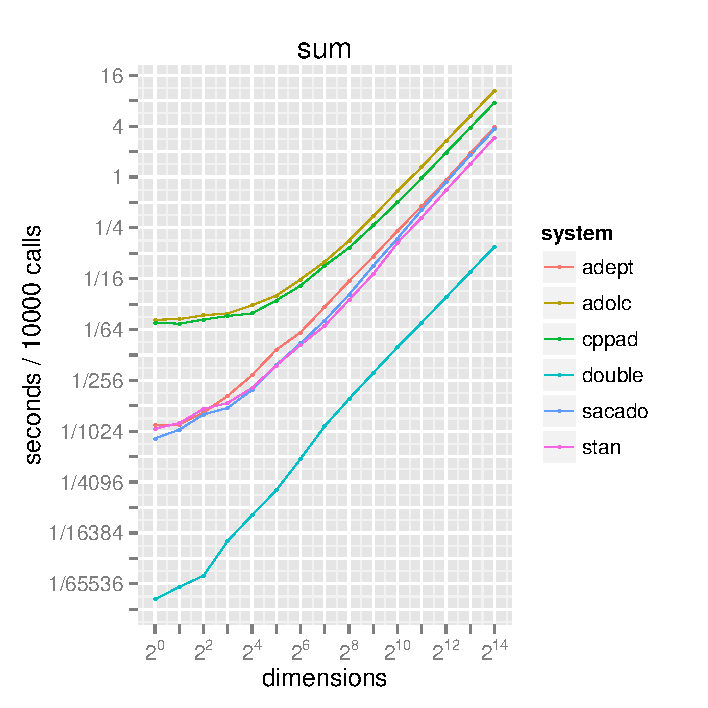
\includegraphics[width=0.48\textwidth]{img/sum_eval.pdf}
\hfill
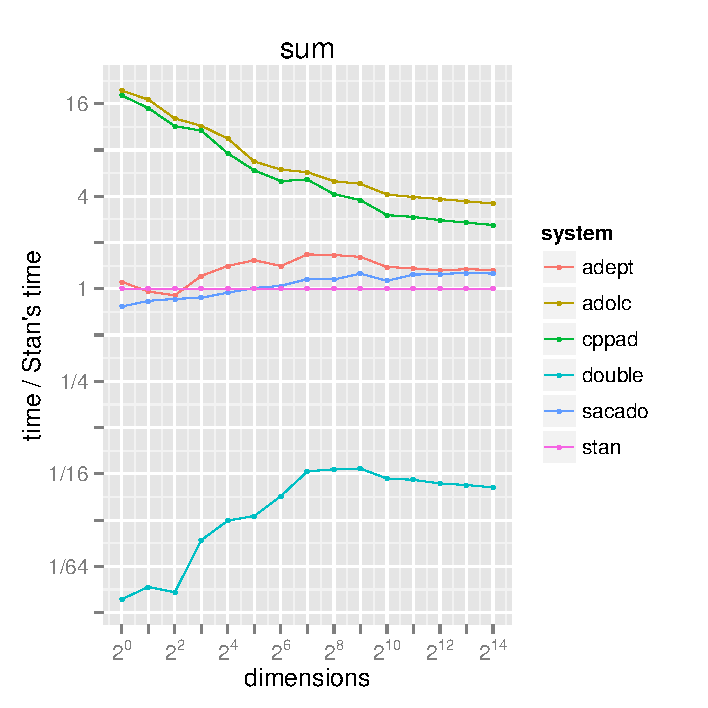
\includegraphics[width=0.48\textwidth]{img/sum_rel_eval.pdf}
\hfill \hfill


\sld{Product \& Log-Sum-Exp}
%
\hfill \hfill
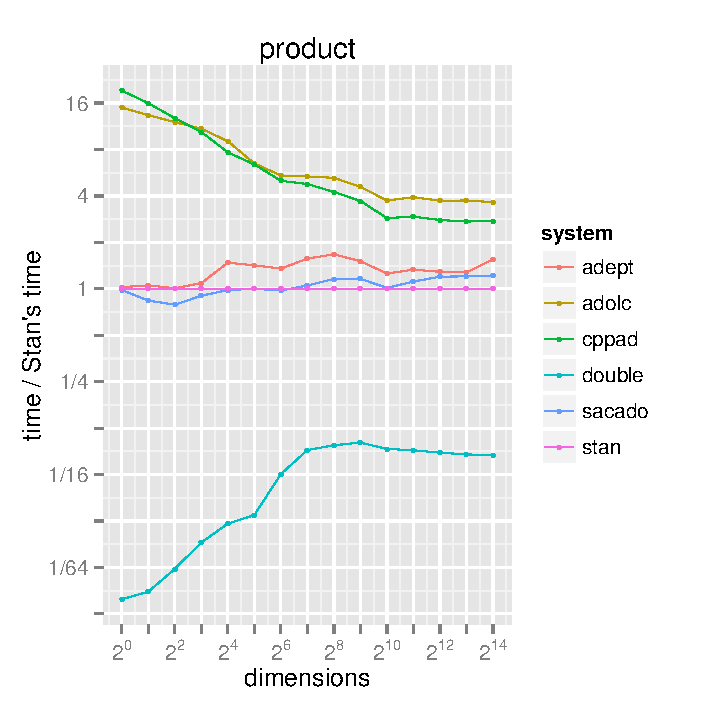
\includegraphics[width=0.45\textwidth]{img/product_rel_eval.pdf}
\hfill
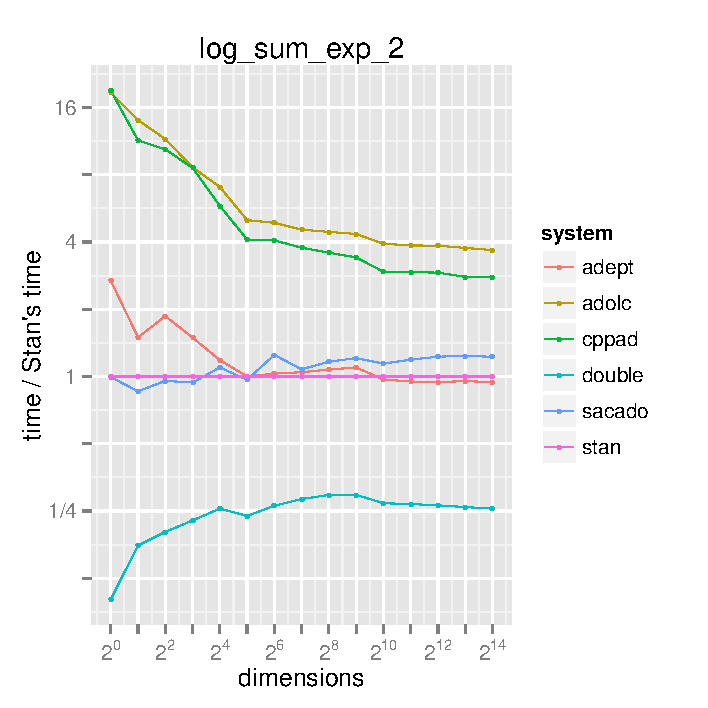
\includegraphics[width=0.45\textwidth]{img/log_sum_exp_2_rel_eval.pdf}
\hfill \hfill


\sld{Stan's Matrix Calculations}
%
\vspace*{-6pt}
\begin{subitemize}
\item Faster in Eigen, but takes more memory
\item Best of both worlds coming soon
\end{subitemize}
\vspace*{-8pt}
\hfill \hfill
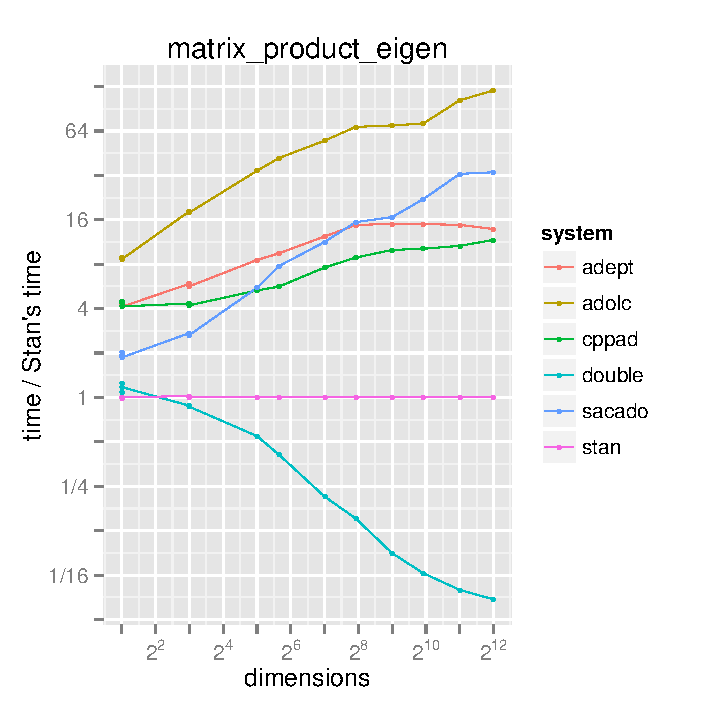
\includegraphics[width=0.48\textwidth]{img/autodiff-eval-matrix-product-eigen.pdf}
\hfill
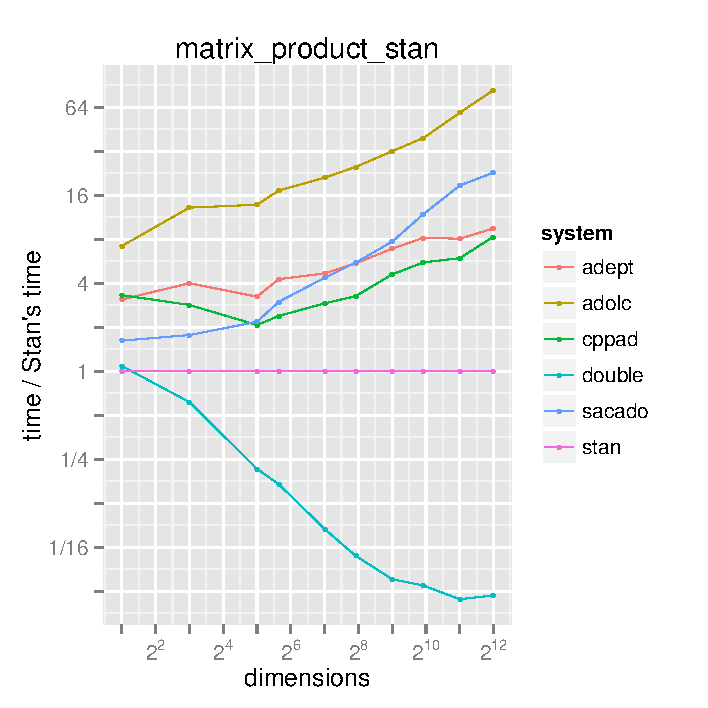
\includegraphics[width=0.48\textwidth]{img/matrix_product_stan_rel_eval.pdf}
\hfill \hfill


\sld{Coding Probability Functions}
%
\begin{itemize}
\item \myemph{Vectorized} to allow scalar or container arguments
  \\ {\footnotesize (containers all same shape; scalars broadcast as necessary)}
\item Avoid \myemph{repeated computations}, e.g. $\log \sigma$ in
  \hspace*{-18pt}
  {\small
    \begin{eqnarray*}
      \textstyle \log \, \mbox{\sf Normal}(y | \mu, \sigma)
      & = & \textstyle \sum_{n=1}^N \log \, \mbox{\sf Normal}(y_n | \mu,\sigma)
      \\[4pt]
      & = & \textstyle \sum_{n=1}^N  - \log \sqrt{2\pi} \ - \log \sigma \ -
      \frac{\textstyle y_n - \mu}{\textstyle 2\sigma^2}
    \end{eqnarray*}
  }
\item recursive \myemph{expression templates} to broadcast and cache scalars,
  generalize containers (arrays, matrices, vectors)
\item \myemph{traits} metaprogram to \myemph{drop constants} (e.g., $-\log
  \sqrt{2 \pi}$ or $\log \sigma$ if constant) 
  and calculate intermediate and return types
\end{itemize}


\sld{Stan's Density Calculations}
%
\begin{itemize}
\item Vectorization a huge win
\end{itemize}
\vspace*{-8pt}
\hfill \hfill
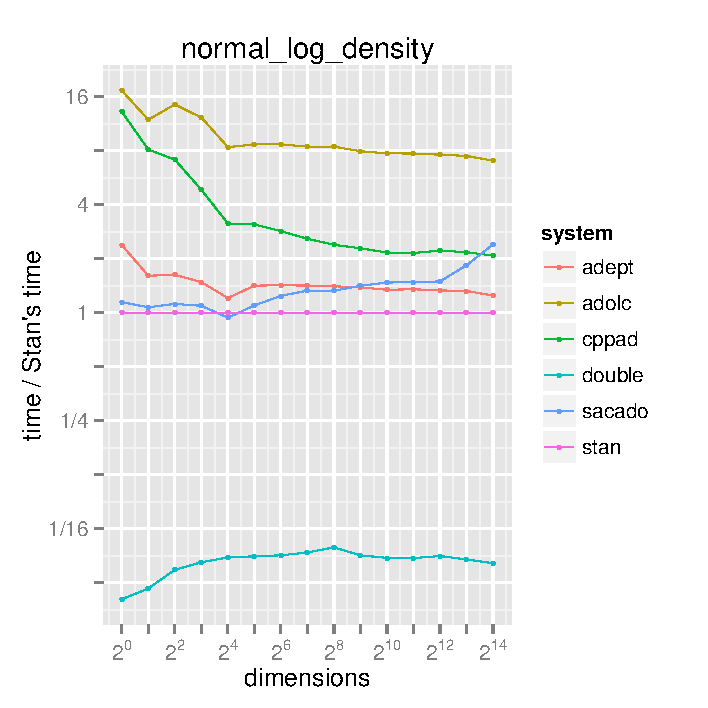
\includegraphics[width=0.48\textwidth]{img/normal_log_density_rel_eval.pdf}
\hfill
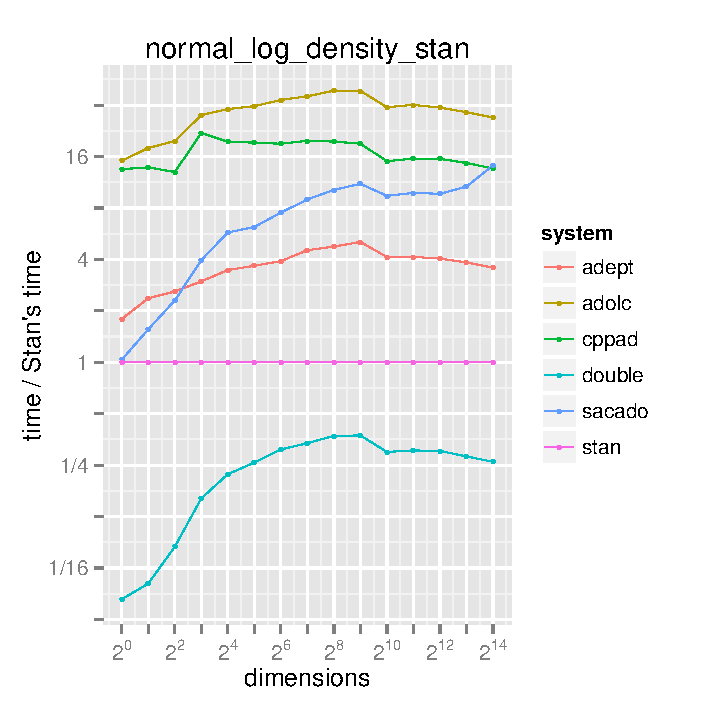
\includegraphics[width=0.48\textwidth]{img/normal_log_density_stan_rel_eval.pdf}
\hfill \hfill


\mypart{Deepr Still}{Autodiff Coding}
%
\sld{Variable Ptr to Impl}
\begin{stancode}
class var {
public:
  var() : vi_(static_cast<vari*>(0U)) { }
  var(double v) : vi_(new vari(v)) { }

  double val() const { return vi_->val_; }
  double adj() const { return vi_->adj_; }  

private:
  vari* vi_;
};
\end{stancode}

\sld{Chainable Base Class}
\begin{stancode}
struct chainable {
  chainable() { }
  virtual ~chainable() { }

  virtual void chain() { }
  virtual void init_dependent() { }
  virtual void set_zero_adjoint() { }

  static inline void* operator new(size_t nbytes) {
    return ChainableStack::memalloc_.alloc(nbytes);
  }
};
\end{stancode}


\sld{Variable Implementation}
%
\begin{stancode}
class vari : public chainable {
public:
  const double val_;
  double adj_;

  vari(double v) : val_(v), adj_(0) { 
    ChainableStack::var_stack_.push_back(this);
  }

  virtual ~vari() { }

  virtual void init_dependent() { adj_ = 1; }
  virtual void set_zero_adjoint() { adj_ = 0; }
};
\end{stancode}


\sld{Memory Management}
%
\begin{stancode}
struct AutodiffStackStorage {
  static std::vector<chainable*> var_stack_;
  static stack_alloc memalloc_;
};

class stack_alloc {
private: 
  std::vector<char*> blocks_;
  std::vector<size_t> sizes_;
  size_t cur_block_;
  char* cur_block_end_;
  char* next_loc_;
  ...
};
\end{stancode}


\sld{Conditional Execution Paths}
%
\begin{stancode}
#ifdef __GNUC__
#define likely(x)      __builtin_expect(!!(x), 1)
#define unlikely(x)    __builtin_expect(!!(x), 0)
#else
#define likely(x)     (x)
#define unlikely(x)   (x)
#endif
\end{stancode}


\sld{Block Allocation}
%
\begin{stancode}
inline void* alloc(size_t len) {
  char* result = next_loc_;
  next_loc_ += len;
  if (unlikely(next_loc_ >= cur_block_end_))
    result = move_to_next_block(len);
  return static_cast<void*>(result);
}
\end{stancode}


\sld{Gradient Calculation}
%
\begin{stancode}
static void grad(chainable* vi) {
  typedef std::vector<chainable*>::reverse_iterator it_t;
  vi->init_dependent(); 
  it_t begin = ChainableStack::var_stack_.rbegin();
  it_t end = ChainableStack::var_stack_.rend();
  for (it_t it = begin; it < end; ++it)
    (*it)->chain();
}
\end{stancode}


\sld{Unary Function}
%
\begin{stancode}
struct op_v_vari : public vari {
  vari* avi_;

  op_v_vari(double f, vari* avi) : vari(f), avi_(avi) { }
};
\end{stancode}

\sld{Logarithm Implementation}
\begin{stancode}
struct log_vari : public op_v_vari {
  log_vari(vari* avi) :
    op_v_vari(std::log(avi->val_), avi) { }

  void chain() {
    avi_->adj_ += adj_ / avi_->val_;
  }
};

inline var log(const var& a) {
  return var(new log_vari(a.vi_));
}
\end{stancode}


\sld{Addition Operator}
%
\begin{stancode}
inline var operator+(const var& a, const var& b) {    
  return var(new add_vv_vari(a.vi_, b.vi_));
}

struct add_vari  ...
  void chain() {
    avi_->adj_ += adj_;
    bvi_->adj_ += adj_;
  }

struct product_vari ...
  void chain() {
    avi_->adj_ += adj_ * b_.val();
    bvi_->adj_ += adj_ * a_.val();
  }
\end{stancode}


\sld{Functor for Function}
%
\begin{stancode}
struct normal_ll {
  const Matrix<double, Dynamic, 1> y_;

  normal_ll(const Matrix<double, Dynamic, 1>& y) : y_(y) { }

  template <typename T>
  T operator()(const Matrix<T, Dynamic, 1>& theta) const {
    T mu = theta[0];   
    T sigma = theta[1];
    T lp = 0;
    for (int n = 0; n < y_.size(); ++n)
      lp += normal_log(y_[n], mu, sigma);
    return lp;
  }
};
\end{stancode}


\sld{Gradient Functional: Use}
%
\begin{stancode}
Matrix<double, Dynamic, 1> y(3);
y << 1.3, 2.7, -1.9;
normal_ll f(y);

Matrix<double, Dynamic, 1> x(2);
x << 1.3, 2.9;

double fx;
Matrix<double, Dynamic, 1> grad_fx;
stan::math::gradient(f, x, fx, grad_fx);
\end{stancode}


\sld{Gradient Functional}
%
\vspace*{-6pt}
\begin{stancode}
template <typename F> 
void gradient(const F& f,  const VectorXd& x,
              double& fx,  VectorXd& grad_fx) {
  try {
    Matrix<var, Dynamic, 1> x_var(x.size());
    for (int i = 0; i < x.size(); ++i) x_var(i) = x(i);
    var fx_var = f(x_var); 
    fx = fx_var.val();
    grad(fx_var.vi_);
    grad_fx.resize(x.size());
    for (int i = 0; i < x.size(); ++i)
      grad_fx(i) = x_var(i).adj();
  } catch (const std::exception& /*e*/) {
    recover_memory();   throw;
  }
  recover_memory();
}
\end{stancode}



\mypart{}{Stan for Big(ger) Data}


\sld{Scaling and Evaluation}
%
\begin{center}
\vspace*{-6pt}
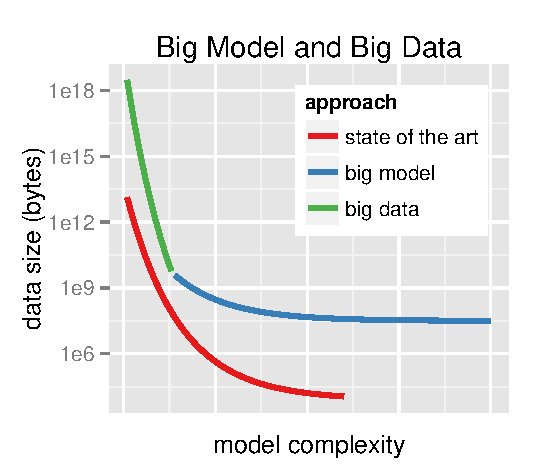
\includegraphics[width=0.6\textwidth]{img/big-model-big-data.pdf}
\vspace*{-6pt}
\end{center}
\begin{itemize}
\item Types of Scaling: data, parameters, \myemph{models}
\end{itemize}


\sld{Riemannian Manifold HMC}
%
\begin{itemize}
\item Best mixing MCMC method (fixed \# of continuous params)
\item Moves on Riemannian manifold rather than Euclidean
\begin{subitemize}
\item adapts to position-dependent curvature
\end{subitemize}
\item \myemph{geoNUTS} generalizes NUTS to RHMC (Betancourt {\slshape arXiv})
\item \myemph{SoftAbs} metric (Betancourt {\slshape arXiv})
\begin{subsubitemize}
\vspace*{-4pt}
\item eigendecompose Hessian and condition
\item computationally feasible alternative to original Fisher info metric
   of Girolami and Calderhead ({\slshape JRSS, Series B})
\item requires third-order derivatives and implicit integrator
\end{subsubitemize}
\vfill
\item merged with develop branch
\end{itemize}


\sld{Maximum Marginal Mode}
%
\begin{itemize}
\item Fast, approx.\ inference for hierarchical models: $p(\phi, \alpha)$
\item Marginalize out lower-level params: $p(\phi) = \int p(\phi, \alpha) d\alpha$
\item Optimize higher-level parameters $\phi^*$ and fix
\item Optimize lower-level parameters given higher-level: $p(\phi^*, \alpha)$
\item Errors estimated as in MLE
\item aka ``empirical Bayes''
\begin{subitemize}
\item but not fully Bayesian
\item and no more empirical than full Bayes
\end{subitemize}
\item Prototypes in R working
\end{itemize}


\sld{Laplace Approximation}
%
\begin{itemize}
\item Multivariate normal approximation to posterior
\item Compute posterior mode via optimization
\[
\theta^{*} = \argmax_{\theta} \  p(\theta | y) 
\]
\item Laplace approximation to the posterior is
\[
p(\theta | y) 
\approx 
\distro{MultiNormal}(\theta^{*} | -H^{-1})
\]
\item $H$ is the Hessian of the log posterior
\[
H_{i,j} 
= \frac{\partial^2}{\partial \theta_i \ \partial \theta_j}
  \log p(\theta | y)
\]
\end{itemize}


\sld{Stan's Laplace Approximation}
%
\begin{itemize}
\item Operates on unconstrained parameters
\item L-BFGS to compute posterior mode $\theta^*$
\item Automatic differentiation to compute $H$
\begin{subitemize}
\item current R: finite differences of gradients
\item soon:  second-order automatic differentiation
\end{subitemize}
\item Draw a sample from approximate posterior
\begin{subitemize}
\item transfrom back to constrained scale
\item allows Monte Carlo computation of expectations
\end{subitemize}
\end{itemize}


\sld{``Black Box'' Variational Inference}
%
\begin{itemize}
%
\item \myemph{Black box} so can fit any Stan model
%
\item Multivariate \myemph{normal approx to unconstrained} posterior
\begin{subitemize}
\item covariance: diagonal mean-field or full rank
\item not Laplace approx --- around posterior mean, not mode
\item transformed back to constrained space (built-in Jacobians)
\end{subitemize}
%
\item Stochastic \myemph{gradient-descent} optimization
\begin{subitemize}
\item ELBO gradient estimated via Monte Carlo + autdiff
\end{subitemize}
%
\item Returns \myemph{approximate posterior} mean / covariance
\item Returns \myemph{sample} transformed to constrained space
\end{itemize}



\sld{VB in a Nutshell}
%
\begin{itemize}
\item $y$ is observed data, $\theta$ parameters
\item Goal is to approximate posterior $p(\theta | y)$
\item with a convenient approximating density $g(\theta | \phi)$
\begin{subitemize}
\item $\phi$ is a vector of parameters of approximating density
\end{subitemize}
\item Given data $y$, VB computes $\phi^*$ 
minimizing KL-divergence
{\small
\begin{eqnarray*}
\phi^* 
& = & 
\displaystyle
\argmin_{\phi} \ \mbox{KL}[g(\theta|\phi) \ || \ p(\theta|y)]
\\[4pt]
& = & 
\displaystyle
\argmin_{\phi}
\int_{\Theta} 
  \log\left(
    \frac{p(\theta \, | \, y)}{g(\theta \, | \, \phi)}
  \right)
  \ g(\theta | \phi) \ \mathrm{d}\theta
\\[4pt]
& = &
\argmin_{\phi} \
\mathbb{E}_{g(\theta|\phi)}\left[\,
  \log p(\theta \, | \, y) - \log g(\theta \, | \, \phi)
\right]
\end{eqnarray*}
}
\end{itemize}


\sld{VB vs.\ Laplace}
%
\vspace*{-6pt}
\begin{center}
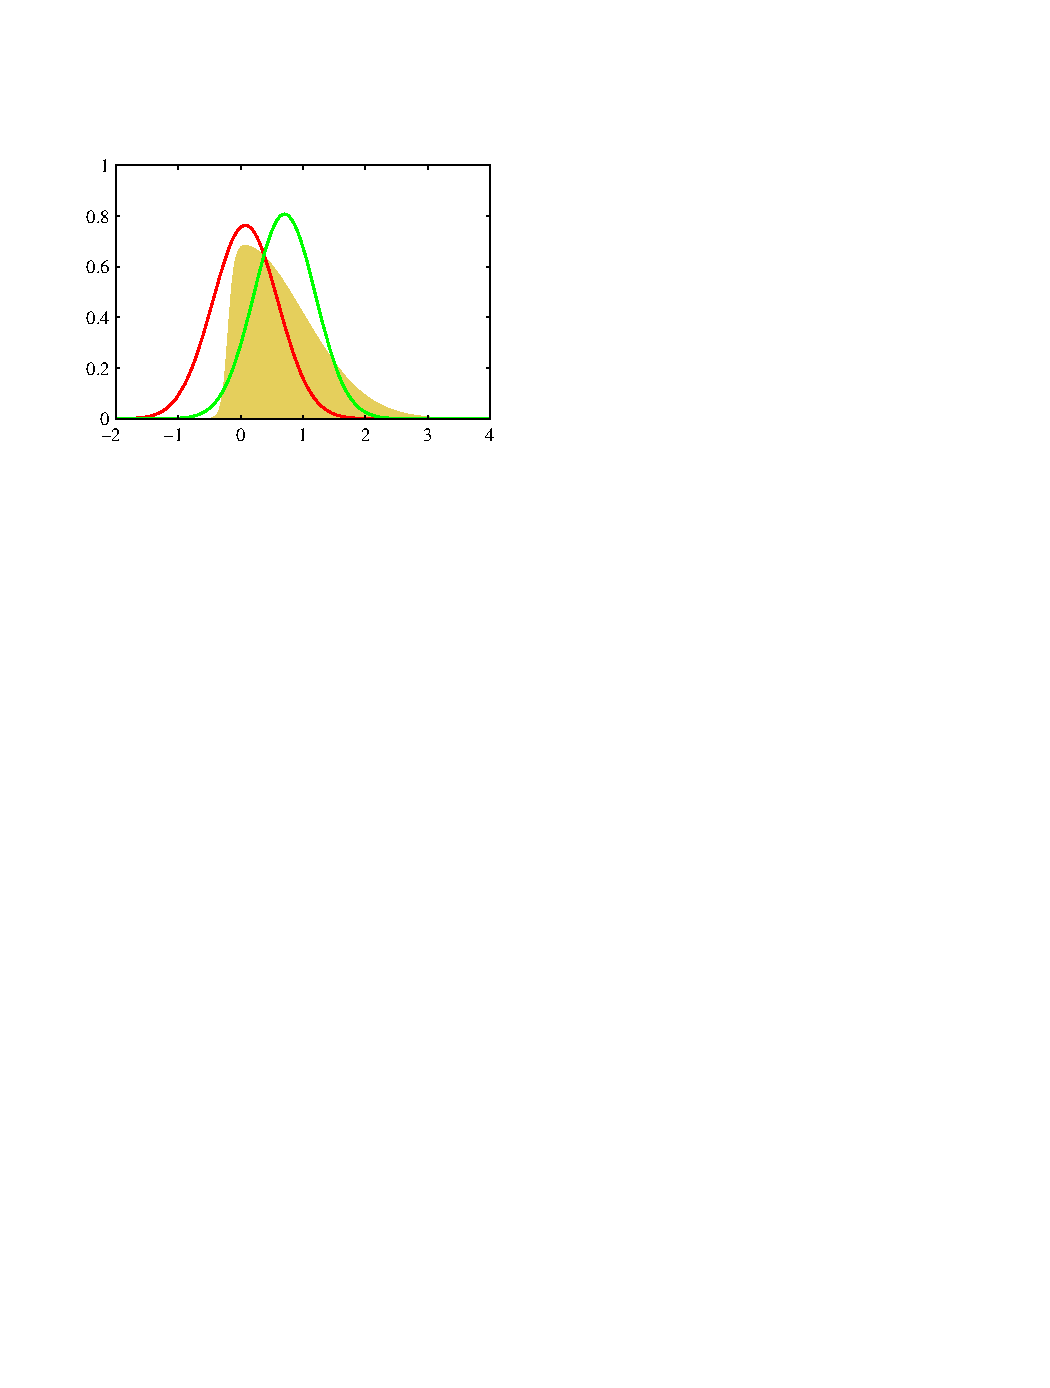
\includegraphics[width=0.45\textwidth]{img/bishop-fig-10-1.pdf}
\end{center}
\vspace*{-10pt}
\begin{itemize}
\item {\slshape solid yellow}: target; \ \ {\slshape red}: Laplace; \ \
  {\slshape green}: VB
\item \myemph{Laplace} located at posterior mode
\item \myemph{VB} located at approximate posterior mean
\end{itemize}
\vfill \hfill
{\footnotesize  --- Bishop (2006) {\slshape Pattern Recognition and Machine Learning}, fig.~10.1}


\sld{KL-Divergence Example}
%
\vspace*{-4pt}
\begin{center}
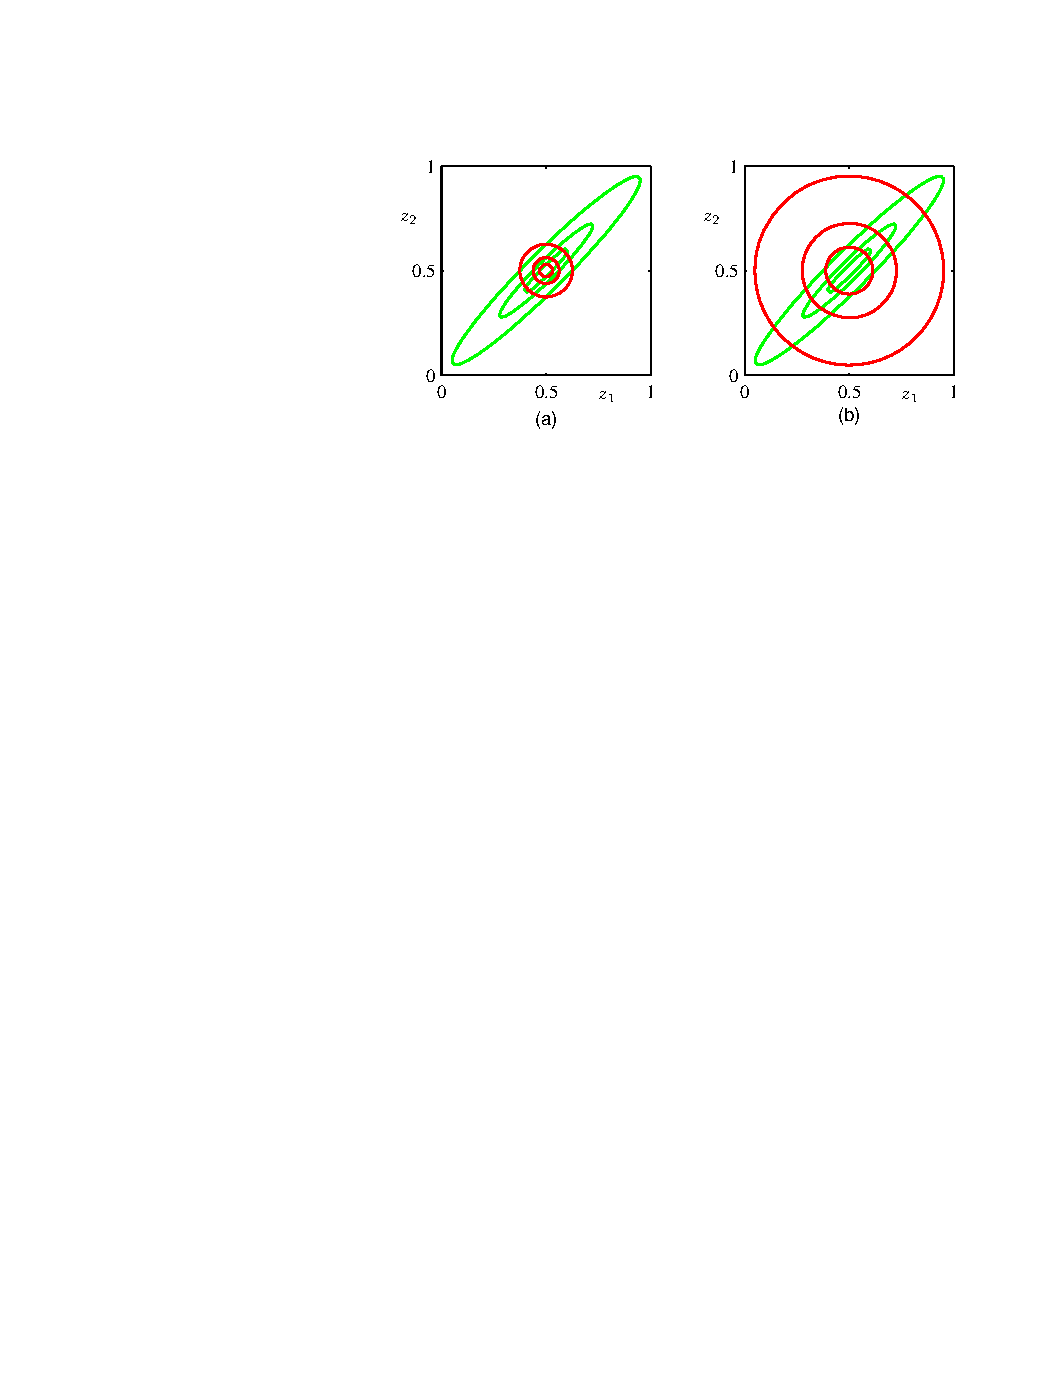
\includegraphics[width=0.6\textwidth]{img/bishop-fig-10-2.pdf}
\end{center}
\vspace*{-10pt}
\begin{subitemize}
\item \myemph{Green}: true distribution $p$; \ \ \myemph{Red}: best
  approximation $g$
\begin{subitemize}
\item[(a)] VB-like: $\mbox{KL}[g \, || \, p]$
\item[(b)] EP-like: $\mbox{KL}[p \, || \, g]$
\end{subitemize}
\item VB systematically \myemph{understimates posterior variance}
\end{subitemize}
\vfill \hfill
{\footnotesize  --- Bishop (2006) {\slshape Pattern Recognition and Machine Learning}, fig.~10.2}


\sld{Stan's ``Black-Box'' VB}
%
\begin{itemize}
\item Typically custom $g()$ per model
\begin{subitemize}
\item based on conjugacy and analytic updates
\end{subitemize}
\item Stan uses ``black-box VB'' with multivariate Gaussian $g$
\[
g(\theta|\phi) = \distro{MultiNormal}(\theta \, | \, \mu, \Sigma)
\]
for the \myemph{unconstrained posterior}
\begin{subitemize}
\item e.g., scales $\sigma$ log-transformed with Jacobian
\end{subitemize}
\item Stan provides two versions
\begin{subitemize}
\item Mean field: $\Sigma$ diagonal
\item General: $\Sigma$ dense
\end{subitemize}
\end{itemize}


\sld{Stan's VB: Computation}
%
\begin{itemize}
\item Use L-BFGS optimization to optimize $\theta$
\item Requires gradient of KL-divergence w.r.t. $\theta$ up to constant
\item Approximate KL-divergence and gradient via Monte Carlo
\begin{subitemize}
\item only need approximate gradient calculation for soundness of L-BFGS
\item KL divergence is an expectation w.r.t. approximation $g(\theta|\phi)$
\item Monte Carlo draws i.i.d.\ from approximating multi-normal
\item derivatives with respect to true model log density via reverse-mode autodiff
\item so only a few Monte Carlo iterations are enough
\end{subitemize}
\end{itemize}

\sld{Stan's VB: Computation (cont.)}
\begin{itemize}
\item To support compatible plug-in inference
\begin{subitemize}
\item draw Monte Carlo sample $\theta^{(1)}, \ldots, \theta^{(M)}$ with
\[
\theta^{(m)} \sim  \distro{MultiNormal}(\theta \, | \, \mu^{*}, \Sigma^{*})
\]
\item inverse transfrom from unconstrained to constrained scale
\item report to user in same way as MCMC draws
\vfill
\end{subitemize}
\item Future: reweight $\theta^{(m)}$ via importance sampling
\begin{subitemize}
\item with respect to true posterior
\item to improve expectation calculations
\end{subitemize}
\end{itemize}


\sld{Near Future: Stochastic VB}
%
\begin{itemize}
\item Data-streaming form of VB 
\begin{subitemize}
\item Scales to billions of observations
\item {\footnotesize Hoffman et al. (2013) Stochastic variational inference. {\slshape JMLR} 14.}
\end{subitemize}
\item Mashup of stochastic gradient (Robbins and Monro 1951) and VB
\begin{subitemize}
\item subsample data (e.g., stream in minibatches)
\item upweight each minibatch to full data set size
\item use to make unbiased estimate of true gradient
\item take gradient step to minimimize KL-divergence
\end{subitemize}
\vfill
\item Prototype code complete
\end{itemize}


\mypart{Part V}{Challenges for Stan}


\sld{Discrete Parameters}
%
\begin{itemize}
\item e.g., simple mixture models, survival models, HMMs,
  discrete measurement error models, missing data
\item \myemph{Marginalize out} discrete parameters
\item Efficient sampling due to \myemph{Rao-Blackwellization}
\item Inference straightforward with expectations
  \vspace*{12pt}
\item Too \myemph{difficult} for many of our users
  \\
  {\small (exploring encapsulation options)}
\end{itemize}


\sld{Models with Missing Data}
%
\begin{itemize}
\item In principle, missing data just \myemph{additional parameters}
\item In practice, how to declare? 
  \begin{itemize}
  \item \myemph{observed} data as data variables
  \item \myemph{missing} data as parameters
  \item combine into single vector 
    \\ {\footnotesize (in transformed parameters or local in model)}
  \end{itemize}
\end{itemize}


\sld{Position-Dependent Curvature}
%
\begin{itemize}
\item Mass matrix does \myemph{global} adaptation for
\begin{subitemize}
\item parameter scale (diagonal) and rotation (dense)
\end{subitemize}
%
\item Dense mass matrices hard to estimate ($\bigoh{N^2}$ estimands)
\item \myemph{Problem}: Position-dependent curvature
\begin{subitemize}
\item Example: banana-shaped densities
\begin{subsubitemize}
\item arise when parameter is product of other parameters
\end{subsubitemize}
\item Example: hierarchical models
\begin{subsubitemize}
\item hierarhcical variance controls lower-level parameters
\end{subsubitemize}
\end{subitemize}
\item Mitigate by reducing stepsize
\begin{subsubitemize}
\item initial (\code{stepsize}) and target acceptance (\code{adapt\_delta})
\end{subsubitemize}
\end{itemize}


\mypart{}{The End}


\end{document}